\documentclass{vkr}
\usepackage[english, russian]{babel} % переносы
\usepackage{graphicx} % для вставки картинок
\graphicspath{{images/}} % путь к изображениям
\usepackage[hidelinks]{hyperref}
\usepackage{float} % определяет метод H для рисунка с переносом на следующую страницу, ели не помещается
\usepackage{pdflscape}
\addto{\captionsrussian}{\renewcommand{\refname}{СПИСОК ИСПОЛЬЗОВАННЫХ ИСТОЧНИКОВ}}
\usepackage{xltabular} % для вставки таблиц
\usepackage{makecell}
\renewcommand\theadfont{} % шрифт в /thead
\usepackage{array} % для определения новых типов столбцов таблиц
\newcolumntype{T}{>{\centering\arraybackslash}X} % новый тип столбца T - автоматическая ширина столбца с выравниванием по центру
\newcolumntype{R}{>{\raggedleft\arraybackslash}X} % новый тип столбца R - автоматическая ширина столбца с выравниванием по правому краю
\newcolumntype{C}[1]{>{\centering\let\newline\\\arraybackslash\hspace{0pt}}m{#1}} % новый тип столбца C - фиксированная ширина столбца с выравниванием по центру
\newcolumntype{r}[1]{>{\raggedleft\arraybackslash}p{#1}} % новый тип столбца r - фиксированная ширина столбца с выравниванием по правому краю
\newcommand{\centrow}{\centering\arraybackslash} % командой \centrow можно центрировать одну ячейку (заголовок) в столбце типа X или p, оставив в оcтальных ячейках другой тип выравнивания
\newcommand{\finishhead}{\endhead\hline\endlastfoot}
\newcommand{\continuecaption}[1]{\captionsetup{labelformat=empty} \caption[]{#1}\\ \hline }
\usepackage{etoolbox}
\AtBeginEnvironment{xltabular}{\refstepcounter{tablecnt}} % подсчет таблиц xltabular, обычные таблицы подсчитываются в классе

\usepackage[tableposition=top]{caption} % подпись таблицы вверху
\captionsetup{strut=off}
\setlength{\intextsep}{0pt} % Vertical space above & below [h] floats
\setlength{\textfloatsep}{0pt} % Vertical space below (above) [t] ([b]) floats
\DeclareCaptionLabelFormat{gostfigure}{Рисунок #2} %подпись рисунка
\DeclareCaptionLabelFormat{gosttable}{Таблица #2} %подпись таблицы
\DeclareCaptionLabelSeparator{gost}{~--~} %разделитель в рисунках и таблицах
\captionsetup{labelsep=gost}
\captionsetup[figure]{aboveskip=10pt,belowskip=4mm,justification=centering,labelformat=gostfigure} % настройка подписи рисунка
\captionsetup[table]{font={stretch=1.41},skip=0pt,belowskip=0pt,aboveskip=8.5pt,singlelinecheck=off,labelformat=gosttable} % настройка подписи таблицы

\setlength{\LTpre}{8mm} % отступ сверху таблицы
\setlength{\LTpost}{6mm} % отступ снизу таблицы

\usepackage{enumitem}
\setlist{nolistsep,wide=\parindent,itemindent=*} % отступы вокруг списков, выравнивание с учетом разделителя

\usepackage{color} %% это для отображения цвета в коде
\usepackage{listings} %% листинги кода
\setmonofont[Scale=0.7]{Verdana} % моноширный шрифт для листинга

\definecolor{codegreen}{rgb}{0,0.6,0}
\definecolor{codegray}{rgb}{0.5,0.5,0.5}
\definecolor{codepurple}{rgb}{0.58,0,0.82}

\lstset{ %
language=C,                 % выбор языка для подсветки (здесь это С)
numbers=left,               % где поставить нумерацию строк (слева\справа)
numberstyle=\tiny,           % размер шрифта для номеров строк
stepnumber=1,                   % размер шага между двумя номерами строк
numbersep=5pt,                % как далеко отстоят номера строк от подсвечиваемого кода
commentstyle=\color{codegreen},
keywordstyle=\color{magenta},
numberstyle=\tiny\color{codegray},
stringstyle=\color{codepurple},
basicstyle=\linespread{0.95}\ttfamily,
backgroundcolor=\color{white}, % цвет фона подсветки - используем \usepackage{color}
showspaces=false,            % показывать или нет пробелы специальными отступами
showstringspaces=false,      % показывать или нет пробелы в строках
showtabs=false,             % показывать или нет табуляцию в строках
frame=single,              % рисовать рамку вокруг кода
tabsize=2,                 % размер табуляции по умолчанию равен 2 пробелам
captionpos=t,              % позиция заголовка вверху [t] или внизу [b] 
breaklines=true,           % автоматически переносить строки (да\нет)
breakatwhitespace=false, % переносить строки только если есть пробел
escapeinside={\%*}{*)}   % если нужно добавить комментарии в коде
}

\makeatletter % чтобы допускались русские комментарии в листингах
\lst@InputCatcodes
\def\lst@DefEC{%
 \lst@CCECUse \lst@ProcessLetter
  ^^80^^81^^82^^83^^84^^85^^86^^87^^88^^89^^8a^^8b^^8c^^8d^^8e^^8f%
  ^^90^^91^^92^^93^^94^^95^^96^^97^^98^^99^^9a^^9b^^9c^^9d^^9e^^9f%
  ^^a0^^a1^^a2^^a3^^a4^^a5^^a6^^a7^^a8^^a9^^aa^^ab^^ac^^ad^^ae^^af%
  ^^b0^^b1^^b2^^b3^^b4^^b5^^b6^^b7^^b8^^b9^^ba^^bb^^bc^^bd^^be^^bf%
  ^^c0^^c1^^c2^^c3^^c4^^c5^^c6^^c7^^c8^^c9^^ca^^cb^^cc^^cd^^ce^^cf%
  ^^d0^^d1^^d2^^d3^^d4^^d5^^d6^^d7^^d8^^d9^^da^^db^^dc^^dd^^de^^df%
  ^^e0^^e1^^e2^^e3^^e4^^e5^^e6^^e7^^e8^^e9^^ea^^eb^^ec^^ed^^ee^^ef%
  ^^f0^^f1^^f2^^f3^^f4^^f5^^f6^^f7^^f8^^f9^^fa^^fb^^fc^^fd^^fe^^ff%
  ^^^^20ac^^^^0153^^^^0152%
  % Basic Cyrillic alphabet coverage
  ^^^^0410^^^^0411^^^^0412^^^^0413^^^^0414^^^^0415^^^^0416^^^^0417%
  ^^^^0418^^^^0419^^^^041a^^^^041b^^^^041c^^^^041d^^^^041e^^^^041f%
  ^^^^0420^^^^0421^^^^0422^^^^0423^^^^0424^^^^0425^^^^0426^^^^0427%
  ^^^^0428^^^^0429^^^^042a^^^^042b^^^^042c^^^^042d^^^^042e^^^^042f%
  ^^^^0430^^^^0431^^^^0432^^^^0433^^^^0434^^^^0435^^^^0436^^^^0437%
  ^^^^0438^^^^0439^^^^043a^^^^043b^^^^043c^^^^043d^^^^043e^^^^043f%
  ^^^^0440^^^^0441^^^^0442^^^^0443^^^^0444^^^^0445^^^^0446^^^^0447%
  ^^^^0448^^^^0449^^^^044a^^^^044b^^^^044c^^^^044d^^^^044e^^^^044f%
  ^^^^0401^^^^0451%
  %%%
  ^^00}
\lst@RestoreCatcodes
\makeatother


% Режим шаблона (должен быть включен один из трех)
\ВКРtrue
%\Практикаtrue
%\Курсоваяtrue

\newcommand{\Дисциплина}{<<Проектирование и архитектура программных систем>>} % для курсовой
\newcommand{\КодСпециальности}{09.03.04} % Курсовая
\newcommand{\Специальность}{Программная инженерия} % Курсовая
\newcommand{\Тема}{Кроссплатформенная система обмена сообщениями} % ВКР Курсовая
\newcommand{\ТемаВтораяСтрока}{}
\newcommand{\ГдеПроводитсяПрактика}{Юго-Западном государственном университете} % для практики
\newcommand{\РуководительПрактПредпр}{Куркина А. В.} % для практики
\newcommand{\ДолжнРуководительПрактПредпр}{директор} % для практики
\newcommand{\РуководительПрактУнивер}{Чаплыгин А. А.} % для практики
\newcommand{\ДолжнРуководительПрактУнивер}{к.т.н. доцент} % для практики
\newcommand{\Автор}{А. С. Пашков}
\newcommand{\АвторРод}{Пашкова А.С.}
\newcommand{\АвторПолностьюРод}{Пашкова Алексея Сергеевича} % для практики
\newcommand{\Шифр}{20-06-0168}
\newcommand{\Курс}{4} % для практики
\newcommand{\Группа}{ПО-01б}
\newcommand{\Руководитель}{Е. А. Петрик} % для ВКР и курсовой
\newcommand{\Нормоконтроль}{А. А. Чаплыгин} % для ВКР
\newcommand{\ЗавКаф}{А. В. Малышев} % для ВКР
\newcommand{\ДатаПриказа}{«04» апреля 2024~г.} % для ВКР
\newcommand{\НомерПриказа}{1620-с} % для ВКР
\newcommand{\СрокПредоставления}{«11» июня 2024~г.} % для ВКР, курсового

\begin{document}
\maketitle
\ifПрактика{}\else{
   \newpage
\begin{center}
\large\textbf{Минобрнауки России}

\large\textbf{Юго-Западный государственный университет}
\vskip 1em
\normalsize{Кафедра программной инженерии}
\vskip 1em
\ifВКР{
        \begin{flushright}
        \begin{tabular}{p{.4\textwidth}}
        \centrow УТВЕРЖДАЮ: \\
        \centrow Заведующий кафедрой \\
        \hrulefill \\
        \setarstrut{\footnotesize}
        \centrow\footnotesize{(подпись, инициалы, фамилия)}\\
        \restorearstrut
        «\underline{\hspace{1cm}}»
        \underline{\hspace{3cm}}
        20\underline{\hspace{1cm}} г.\\
        \end{tabular}
        \end{flushright}
        }\fi
\end{center}
\vspace{1em}
  \begin{center}
  \large
\ifВКР{
ЗАДАНИЕ НА ВЫПУСКНУЮ КВАЛИФИКАЦИОННУЮ РАБОТУ
  ПО ПРОГРАММЕ БАКАЛАВРИАТА}
  \else
ЗАДАНИЕ НА КУРСОВУЮ РАБОТУ (ПРОЕКТ)
\fi
\normalsize
  \end{center}
\vspace{1em}
{\parindent0pt
  Студента \АвторРод, шифр\ \Шифр, группа \Группа
  
1. Тема «\Тема\ \ТемаВтораяСтрока»
\ifВКР{
утверждена приказом ректора ЮЗГУ от \ДатаПриказа\ № \НомерПриказа
}\fi.

2. Срок предоставления работы к защите \СрокПредоставления

3. Исходные данные для создания программной системы:

3.1. Перечень решаемых задач:}

\renewcommand\labelenumi{\theenumi)}

\begin{enumerate}
\item проанализировать предметную область, определить особенности аналогичных приложений и рассмотреть виды приложений данного типа;
\item  разработать концептуальную модель программной системы обмена сообщениями;
\item спроектировать архитектуру разрабатываемой системы;
\item сконструировать програмную систему, произвести ее системное тестирование.
\end{enumerate}

{\parindent0pt
  3.2. Входные данные и требуемые результаты для программы:}

\begin{enumerate}
\item Входными данными для программной системы являются: пользовательские данные, сообщения пользователей и загружаемые медиа-файлы.
\item Выходными данными для программной системы являются: непосредственные выходные данные в разрабатываемой системе отсутствуют.
\end{enumerate}

{\parindent0pt

  4. Содержание работы (по разделам):
  
  4.1. Введение
  
  4.1. Анализ предметной области
  
4.2. Техническое задание: основание для разработки, назначение разработки,
требования к программной системе, требования к оформлению документации.

4.3. Технический проект: общие сведения о программной системе, проект
данных программной системы, проектирование архитектуры программной системы, проектирование пользовательского интерфейса программной системы.

4.4. Рабочий проект: спецификация компонентов и классов программной системы, тестирование программной системы, сборка компонентов программной системы.

4.5. Заключение

4.6. Список использованных источников

5. Перечень графического материала:

\списокПлакатов

\vskip 2em
\begin{tabular}{p{6.8cm}C{3.8cm}C{4.8cm}}
Руководитель \ifВКР{ВКР}\else работы (проекта) \fi & \lhrulefill{\fill} & \fillcenter\Руководитель\\
\setarstrut{\footnotesize}
& \footnotesize{(подпись, дата)} & \footnotesize{(инициалы, фамилия)}\\
\restorearstrut
Задание принял к исполнению & \lhrulefill{\fill} & \fillcenter\Автор\\
\setarstrut{\footnotesize}
& \footnotesize{(подпись, дата)} & \footnotesize{(инициалы, фамилия)}\\
\restorearstrut
\end{tabular}
}

\renewcommand\labelenumi{\theenumi.}

   \abstract{РЕФЕРАТ}

Объем работы равен \formbytotal{lastpage}{страниц}{е}{ам}{ам}. Работа содержит \formbytotal{figurecnt}{иллюстраци}{ю}{и}{й}, \formbytotal{tablecnt}{таблиц}{у}{ы}{}, \arabic{bibcount} библиографических источников и \formbytotal{числоПлакатов}{лист}{}{а}{ов} графического материала. Количество приложений – 2. Графический материал представлен в приложении А. Фрагменты исходного кода представлены в приложении Б.

Перечень ключевых слов: веб-приложение, чат-приложение, ASP.NET Core, Next.js, серверная часть, клиентская часть, веб-разработка, JavaScript, React, Универсальное приложение, серверный рендеринг, статическая генерация страниц, динамическое обновление, маршрутизация, REST API, авторизация и аутентификация, пользовательский интерфейс, фронтенд, бэкенд, компонентная архитектура, взаимодействие клиента и сервера, безопасность данных, масштабируемость, производительность, тестирование.

Объектом разработки является веб-приложение, обеспечивающее коммуникацию пользователей приложения посредством обмена сообщениями внури чат-комнат.

Целью выпускной квалификационной работы является обеспечение заинтересованных пользователей сервисом, который будет позволять им общаться через глобальную сеть Интернет.

В ходе разработки приложения были выявлены ключевые элементы, которые были организованы в виде информационных блоков. Для эффективной работы с этими элементами были использованы классы и методы соответствующих модулей, обеспечивая связь с сущностями предметной области. Кроме того, были спроектированы и внедрены разделы, необходимые для обеспечения внутренней коммуникации между пользователями в рамках приложения, гарантируя тем самым корректное функционирование веб-сайта.


\selectlanguage{english}
\abstract{ABSTRACT}
  
The volume of work is \formbytotal{lastpage}{page}{}{s}{s}. The work contains \formbytotal{figurecnt}{illustration}{}{s}{s}, \formbytotal{tablecnt}{table}{}{s}{s}, \arabic{bibcount} bibliographic sources and \formbytotal{числоПлакатов}{sheet}{}{s}{s} of graphic material. The number of applications is 2. The graphic material is presented in annex A. The layout of the site, including the connection of components, is presented in annex B.

List of key words: web application, chat application, ASP.NET Core, Next.js, server-side, client-side, web development, JavaScript, React, Universal application, server-side rendering, static page generation, dynamic updating, routing, REST API, authentication and authorization, user interface, frontend, backend, component-based architecture, client-server interaction, data security, scalability, performance, testing.

The object of development is a web application facilitating user communication through message exchange within chat rooms.

The aim of the final qualification work is to provide interested users with a service that will allow them to communicate via the global Internet.

During the application development process, key elements were identified, organized as informational blocks. Classes and methods of corresponding modules were utilized to effectively work with these elements, ensuring connectivity with domain entities. Additionally, sections necessary for internal communication between users within the application were designed and implemented, thereby guaranteeing the correct functioning of the website.
\selectlanguage{russian}
}\fi
\tableofcontents
\section*{ОБОЗНАЧЕНИЯ И СОКРАЩЕНИЯ}

БД -- база данных.

ИС -- информационная система.

ИТ -- информационные технологии. 

КТС -- комплекс технических средств.

ОМТС -- отдел материально-технического снабжения. 

ПО -- программное обеспечение.

РП -- рабочий проект.

СУБД -- система управления базами данных.

ТЗ -- техническое задание.

ТП -- технический проект.

UML (Unified Modelling Language) -- язык графического описания для объектного моделирования в области разработки программного обеспечения.

\ifПрактика{}\else{\section*{ВВЕДЕНИЕ}
\addcontentsline{toc}{section}{ВВЕДЕНИЕ}

В современном мире, где цифровые технологии проникают во все сферы жизни, веб-приложения становятся неотъемлемой частью повседневного общения и взаимодействия людей. Одним из наиболее востребованных типов веб-приложений является чат, позволяющий пользователям обмениваться сообщениями в реальном времени. Такие приложения находят широкое применение как в личной, так и в профессиональной сфере, обеспечивая оперативное общение, координацию и совместную работу.

Разработка веб-приложения чата представляет собой сложный и многогранный процесс, включающий в себя выбор подходящих технологий, проектирование архитектуры системы, реализацию функциональных компонентов и обеспечение безопасности данных. Успешное создание такого приложения требует не только глубоких знаний и навыков в области веб-разработки, но и понимания особенностей и требований пользователей, а также современных трендов в сфере информационных технологий.

\emph{Цель данной работы} заключается в создании веб-приложения, обеспечивающего возможность пользователей обмениваться сообщениями в чат-комнатах. Для достижения этой цели необходимо разработать серверную часть приложения, предоставляющую возможность независимо от нее разрабатывать различные клиенты для разных платформ. Для этого необходимо решить следующие задачи:

\begin{itemize}
	\item разработать требования к программной системе; определить модель данных и варианты использования;
	\item спроектировать архитектуру программной системы; определить маршруты приложения; произвести выбор технологий для программной реализации;
	\item реализовать модули программной системы с использованием выбранных технологий; реализовать пользовательский интерфейс в виде веб-сайта для демонстрации работы приложения; провести системное тестирование программной системы. 
\end{itemize}

\emph{Структура и объем работы.} Отчет состоит из введения, 4 разделов основной части, заключения, списка использованных источников, 2 приложений. Текст выпускной квалификационной работы равен 153 страницам.

\emph{Во введении} сформулирована цель работы, поставлены задачи разра-
ботки, описана структура работы, приведено краткое содержание каждого из разделов.

\emph{В первом разделе} приводится анализ предметной области, рассмотрено понятие чата, роль чатов в обществе, их основные виды и история развития. 

\emph{Во втором разделе} на определяются требования к разрабатываемой программной системе.

\emph{В третьем разделе} на стадии технического проектирования представленf архитектура программнойсистемы.

\emph{Четвертый этап} представляет собой рабочий проект. В этом разделе описаны классы приложения, их поля и методы. Также здесь приведены результаты системного тестирования программной системы.

\emph{В заключении} описаны результаты проведенной работы.

В приложении А представлен графический материал.
В приложении Б содержатся фрагменты исходного кода созданной
программно-информационной системы}\fi
\section{Анализ предметной области}
\subsection{Понятие чата и роль чатов в обществе}

Чат, в своей простейшей форме, означает обмен сообщениями в реальном времени между двумя или более пользователями через интернет. Однако его значение выходит далеко за пределы простого текстового общения, охватывая широкий спектр методов общения, платформ и функциональных возможностей.

В своей сути чат служит фундаментальным инструментом для создания связей и формирования сообществ в цифровом мире. От приложений мгновенного обмена сообщениями до социальных медиа и онлайн-форумов, чат обеспечивает безпрепятственное общение и сотрудничество вне зависимости от географических границ, часовых поясов и культурных барьеров. Он позволяет людям вести беседы, делиться идеями, выражать эмоции и устанавливать отношения с другими, независимо от физического расстояния.

Одной из ключевых ролей чата в интернет-пространстве является его способность улучшать связь и сокращать расстояние между людьми, бизнесом и организациями. Через платформы чата люди могут общаться в одиночку, участвовать в групповых обсуждениях или публичных форумах, способствуя обмену знаниями, сетевым связям и социальному взаимодействию. Будь то встречи с друзьями, совместная работа над проектами с коллегами, получение клиентской поддержки или участие в онлайн-сообществах, чат предоставляет гибкую и доступную среду для общения.

Кроме того, чат играет важную роль в различных сферах жизни, включая образование, развлечения, коммерцию и здравоохранение. В образовании платформы на основе чата позволяют студентам и преподавателям участвовать в виртуальных классах, обсуждениях и учебных группах, способствуя дистанционному обучению и сотрудничеству. В области развлечений функции онлайн-чата позволяют аудитории взаимодействовать с создателями контента, участвовать в прямых трансляциях и делиться своими мыслями в реальном времени.

В сфере коммерции чат стал мощным инструментом для обслуживания клиентов, продаж и поддержки. Чат-боты и виртуальные ассистенты предоставляют автоматизированную помощь, отвечают на вопросы и облегчают транзакции, улучшая опыт клиента и стимулируя рост бизнеса. Кроме того, платформы на основе чата служат виртуальными рынками, позволяя пользователям легко покупать, продавать и обменивать товары и услуги.

\subsection{История развития чатов и их будущее}

История развития чат-приложений начинается задолго до эпохи смартфонов и мобильного интернета. В 1970-1980-х годах появились первые прототипы, предшествующие современным мессенджерам. Один из таких примеров - команда Unix "talk", позволявшая пользователям обмениваться текстовыми сообщениями в реальном времени на одной системе. Несмотря на свою ограниченность и локальность, это был значимый шаг в направлении онлайн-коммуникаций.

Следующим важным этапом стало появление Internet Relay Chat (IRC) в конце 1980-х и начале 1990-х годов. IRC представлял собой протокол для групповых обсуждений и создания чат-комнат, что сделало онлайн-общение более доступным и интерактивным.

Однако настоящий перелом в истории чат-приложений произошел с появлением AOL Instant Messenger (AIM) в 1997 году. AIM предложил пользовательские профили, списки друзей, а также возможность обмена файлами, что привлекло миллионы пользователей по всему миру и сделало мессенджер популярным средством общения.

В начале 2000-х годов MSN Messenger и Yahoo Messenger стали лидерами рынка чат-приложений, предлагая широкий набор функций, включая мгновенные сообщения, голосовые и видео вызовы, а также возможность обмена файлами. Эти приложения стали неотъемлемой частью повседневной интернет-культуры того времени.

С развитием смартфонов и мобильного интернета в начале 2000-х годов чат-приложения стали доступны на всех типах устройств, открывая новые горизонты для коммуникации. WhatsApp и WeChat были одними из первых мессенджеров, адаптированных для мобильных устройств, и быстро завоевали популярность благодаря своей удобной и многофункциональной платформе.

В настоящее время чат-приложения представляют собой сложные платформы с разнообразными функциями, включая голосовые и видеовызовы, стикеры, GIF-анимации, ботов и интеграцию с другими сервисами. Платформы, такие как Facebook Messenger, Telegram, Signal и Discord, являются примерами современных чат-приложений, предлагающих широкий спектр возможностей для общения и взаимодействия.

Будущее чат-приложений обещает множество инноваций, включая развитие технологий искусственного интеллекта, виртуальной и дополненной реальности. Однако, вместе с этим возрастает и важность вопросов конфиденциальности и безопасности данных, что стимулирует инновации в области шифрования и защиты личной информации.

\subsection{Виды чатов и их особенности}

Существуют различные виды приложений-чатов. Каждый вид обеспечивает конечного пользователя необходимыми функциями и средствами для общения в опрделенном формате или в определенной сфере деятельности. Ниже приведен список основных видов чат-приложений.

\begin{enumerate}
	\item Приложения для обмена сообщениями "один на один":
	
	Приложения для обмена сообщениями "один на один" предназначены для приватных разговоров между двумя пользователями. Эти приложения ориентированы на простоту и конфиденциальность, предлагая такие функции, как текстовые сообщения, голосовые звонки и видеочаты. Примеры включают WhatsApp, Facebook Messenger и Apple iMessage.
	
	\item Платформы для группового чата:
	
	Платформы для группового чата позволяют нескольким пользователям взаимодействовать в разговорах в общем виртуальном пространстве. Эти приложения идеально подходят для координации групповых мероприятий, планирования событий или обсуждения общих интересов. Популярные примеры включают Slack, Discord и Microsoft Teams.
	
	\item Приложения для обмена сообщениями в социальных сетях:
	
	Платформы социальных сетей часто интегрируют функции обмена сообщениями для облегчения общения между пользователями. Эти приложения позволяют отправлять личные сообщения, делиться записями и участвовать в групповых чатах в контексте своей социальной сети. Примерами явлются Facebook Messenger, Instagram Direct Messages и Twitter Direct Messages.
	
	\item Инструменты для совместной работы команд:
	
	Инструменты для совместной работы команд нацелены на профессиональные среды, предлагая продвинутые функции для управления проектами, обмена файлами и интеграции рабочего процесса. Эти приложения упрощают коммуникацию между членами команды, обеспечивая беспрепятственное сотрудничество над задачами и проектами. Примеры: Slack, Microsoft Teams и Asana.
	
	\item Приложения для обмена анонимными сообщениями:
	
	Приложения для обмена анонимными сообщениями позволяют пользователям общаться без раскрытия своей личности. Эти приложения могут предоставлять анонимные чаты, где пользователи могут делиться своими мыслями и чувствами без страха судейства или ограничений. Примерами могут служить Sarahah, Whisper и Yik Yak (хотя последнее приложение уже неактивно).
	
	\item Приложения для обмена короткими видео и аудиосообщениями:
	
	Приложения для обмена короткими видео и аудиосообщениями сосредотачиваются на мультимедийном контенте, позволяя пользователям создавать и обмениваться короткими видеороликами или голосовыми сообщениями. Примерами таких приложений могут служить TikTok, Instagram Direct Messages и WhatsApp Status. Эти приложения становятся все более популярными в мире, где пользователи все больше стремятся к моментальному обмену информацией в удобной форме.
	
	\item Приложения для анонимных групповых чатов:
	
	Приложения для анонимных групповых чатов предоставляют платформу для общения в группах, где участники остаются анонимными. Эти приложения позволяют пользователям присоединяться к обсуждениям по различным темам, не раскрывая своей личности или идентификации, например Discord-серверы с анонимным доступом и Reddit-чаты.
	
	\item Приложения для обмена сообщениями с использованием шифрования:
	
	Приложения для обмена сообщениями с использованием шифрования обеспечивают высокий уровень конфиденциальности и безопасности сообщений между пользователями. Эти приложения используют современные шифровальные методы для защиты данных и обеспечивают конфиденциальность обмена сообщениями. Примеры включают Signal, Telegram и WhatsApp.
\end{enumerate}
\section{Техническое задание}
\subsection{Основание для разработки}

Основанием для разработки является задание на выпускную квалификационную работу бакалавра "<Кроссплатформенная система обмена сообщениями">.

\subsection{Цель и назначение разработки}

Разрабатываемый программный продукт предназначен для организации общения пользователей приложения.

Пользователи данного приложения должны иметь возможность создавать свои комнаты для общения, управлять пользователями комнаты в соответствии со своими ролями, обмениваться голосовыми и текстовыми сообщениями, а также иметь возможность отправлять файлы.

Задачами данной разработки являются:
\begin{itemize}
\item проектирование архитектуры приложения;
\item реализация функциональности серверной части приложения;
\item реализация механизмов аутентификации и авторизации;
\item реализация клиентской части приложения;
\item тестирование и отладка.
\end{itemize}


\subsection{Функциональные требования к программной системе}

Для неавторизованных пользователей системы должны быть доступны следующие функции:

\begin{itemize}
	\item вход в приложение,
	\item регистрация.
\end{itemize}

Вне чат-комнаты авторизованным пользователям должны быть доступны следующие функции:
\begin{itemize}
	\item создание чат-комнаты,
	\item управление личными данными.
\end{itemize}
Внутри чат-комнаты предусмотрено наличие трех классов пользователей: администраторы чата, модераторы чата и обычные пользователи.

Администратором чата назначается пользователь, создавший чат. Он должен иметь следующие возможности:
\begin{itemize}
	\item добавление новых пользователей,
	\item удаление пользователей,
	\item удаление сообщений,
	\item удаление чата,
	\item управление ролями пользователей,
	\item отправка сообщений и файлов,
	\item редактирование своих сообщений.
\end{itemize}

Модераторы чата имеют те же возможности, что и администраторы, за исключением возможностей управления ролями пользователей и удаления чата.

Функции, доступные обычному пользователю:
\begin{itemize}
	\item добавление новых пользователей,
	\item удаление своих сообщений,
	\item отправка сообщений и файлов,
	\item редактирование своих сообщений.
\end{itemize}

\subsection{Моделирование вариантов использования}

Учитывая описанные ранее функцианальные требования к программной системе можно разработать модель вариантов использования системы.

Для составления данной модели используется язык визуального моделирования UML.

Данная описывает взаимодействие пользователей (актеров) с системой через варианты использования (use cases) для достижения определенной цели. В диаграмме выделяются актёры, варианты использования и связи между ними. Актёры представляют внешние сущности, взаимодействующие с системой, и обозначаются человечками или именем актёра. Варианты использования описывают функции или задачи системы и обозначаются овальными фигурами. Связи между актёрами и вариантами использования показывают, кто инициирует или участвует в конкретном варианте использования, и обозначаются линиями. Дополнительные элементы включают обобщение актёров, включение, расширение и системные границы, которые помогают уточнить и организовать функциональные требования системы. 

На рисунке \ref{unauth:image} в виде диаграммы прецедентов представлены функциональные требования к системе для неавторизованных пользователей.

На рисунке \ref{auth:image} в виде диаграммы прецедентов представлены функциональные требования к системе для авторизованных пользователей вне чат-комнаты.

На рисунке \ref{admin:image} в виде диаграммы прецедентов представлены функциональные требования к системе для авторизованных пользователей внутри чат комнаты для роли администратора чата. Построение отдельных диаграмм для остальных ролей не требуется, т.к. все прецеденты будут отражены на диаграмме прецедентов для роли администратора.

\begin{figure}[ht]
	\center{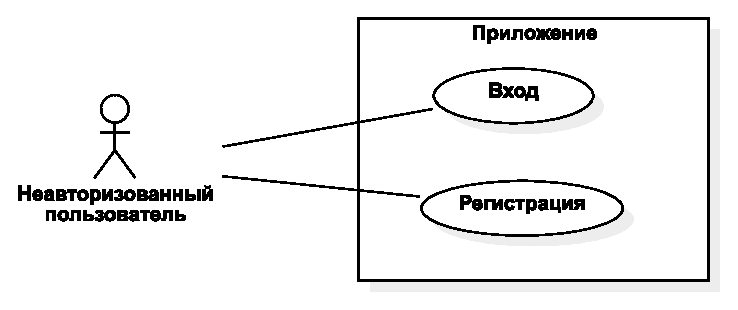
\includegraphics[width=1\linewidth]{unauth}}
	\caption{Диаграмма компонентов}
	\label{unauth:image}
\end{figure}
\ \\
\begin{figure}[ht]
	\center{\includegraphics[width=1\linewidth]{auth}}
	\caption{Диаграмма компонентов}
	\label{auth:image}
\end{figure}

\begin{figure}[H]
	\center{\includegraphics[width=1\linewidth]{admin}}
	\caption{Диаграмма компонентов}
	\label{admin:image}
\end{figure}

\subsubsection{Вариант использования "<Вход в приложение">}

Заинтересованные лица и их требования: пользователи, желающие получить доступ к функционалу приложения.

Предусловие: пользователь открыл приложение и находится на экране входа, пользователь зарегистрирован в приложении.

Постусловие: после успешной авторизации пользователь получает доступ к функциям приложения.

Основной успешный сценарий:
\begin{enumerate}
	\item Пользователь открывает приложение и переходит на экран входа.
	\item Пользователь вводит свои учетные данные (логин и пароль) в соответствующие поля.
	\item Приложение проверяет введенные учетные данные на корректность.
	\item При успешной проверке приложение авторизует пользователя и перенаправляет его на главный экран приложения.
\end{enumerate}

\subsubsection{Вариант использования "<Регистрация">}

Заинтересованные лица и их требования: пользователи, желающие получить доступ к функционалу приложения.

Предусловие: пользователь открыл приложение и находится на экране регистрации, пользователь не зарегистрирован в приложении.

Постусловие: пользователь получает доступ к созданной им чат-комнате.

Основной успешный сценарий:

\begin{enumerate}
	\item Пользователь запускает приложение и переходит на экран регистрации.
	\item Пользователь вводит нкобходимые для регистрации данные.
	\item Приложение проверяет введенные данные на корректность и уникальность.
	\item При успешной проверке приложение создает новую учетную запись для пользователя.
	\item Пользователь получает подтверждение успешной регистрации и может авторизоваться в системе используя свои учетные данные.
\end{enumerate}

\subsubsection{Вариант использования "<Создание чат-комнаты">}

Заинтересованные лица и их требования: пользователь хочет создать собственную чат-комнату для общения.

Предусловие: пользователь открыл приложение и находится на основном экране приложения, пользователь успешно прошел авторизацию.

Постусловие: после успешной регистрации пользователь получает доступ к функциям приложения.

Основной успешный сценарий:

\begin{enumerate}
	\item Пользователь открывает главный экран приложения.
	\item Пользователь выбирает опцию "Создать чат-комнату".
	\item Пользователь вводит название и указывает необходимые параметры.
	\item Приложение проверяет корректность введенных данных и создает новую чат-комнату.
	\item После успешного создания комнаты пользователь автоматически перенаправляется в нее.
\end{enumerate}

\subsubsection{Вариант использования "<Управление личными данными">}

Заинтересованные лица и их требования: пользователь хочет изменить свои данные, указанные при регистрации в приложении.

Предусловие: пользователь открыл приложение и находится в личном кабинете, пользователь успешно прошел авторизацию.

Постусловие: данные пользователя успешно изменены.

Основной успешный сценарий:

\begin{enumerate}
	\item Пользователь открывает главный экран приложения.
	\item Пользователь выбирает опцию "Страница пользователя".
	\item Пользователь производит необходимые изменения.
	\item Приложение проверяет корректность введенных данных и сохраняет изменения.
	\item Пользователь видит новые данные у себя на странице.
\end{enumerate}

\subsubsection{Вариант использования "<Добавление нового пользователя">}

Заинтересованные лица и их требования: пользователь хочет добавить нового участника в чат-комнату.

Предусловие: пользователь открыл приложение и находится в чат-комнате, пользователь успешно прошел авторизацию.

Постусловие: новый пользователь добавлен в чат-комнату.

Основной успешный сценарий:

\begin{enumerate}
	\item Пользователь открывает приложение и заходит в одну из доступных чат-комнат.
	\item Пользователь выбирает опцию "Добавить пользователя".
	\item Пользователь выбирает другого пользователя, которого хочет добавить в чат-комнату.
	\item Новый пользователь добавлен в чат-комнату.
\end{enumerate}

\subsubsection{Вариант использования "<Удаление пользователя">}

Заинтересованные лица и их требования: пользователь хочет удалить участника из чат-комнаты.

Предусловие: пользователь открыл приложение и находится в чат-комнате, пользователь успешно прошел авторизацию и имеет роль либо администратора, либо модератора.

Постусловие: выбранный пользователь удален из чат-комнаты.

Основной успешный сценарий:

\begin{enumerate}
	\item Пользователь открывает приложение и заходит в одну из доступных чат-комнат.
	\item Пользователь выбирает участника чата, которого хочет удалить и выбирает опцию "<Удалить пользователя">.
	\item Пользователь подтверждает свой выбор.
	\item Выбранный пользователь удален из чат-комнаты.
\end{enumerate}

\subsubsection{Вариант использования "<Удаление сообщения">}

Заинтересованные лица и их требования: пользователь хочет удалить свое сообщение в чате.

Предусловие: пользователь открыл приложение и находится в чат-комнате, пользователь успешно прошел авторизацию.

Постусловие: выбранное сообщение удалено из чата.

Основной успешный сценарий:

\begin{enumerate}
	\item Пользователь открывает приложение и заходит в одну из доступных чат-комнат.
	\item Пользователь выбирает сообщение, которое хочет удалить и выбирает опцию "<Удалить сообщение">.
	\item Пользователь подтверждает свой выбор.
	\item Выбранное сообщение удалено из чата.
\end{enumerate}

\subsubsection{Вариант использования "<Управление ролями пользователя">}

Заинтересованные лица и их требования: пользователь хочет изменить роль участника чат-комнаты.

Предусловие: пользователь открыл приложение и находится в чат-комнате, пользователь успешно прошел авторизацию и имеет роль администратора.

Постусловие: роль выбранного пользователя изменена.

Основной успешный сценарий:

\begin{enumerate}
	\item Пользователь открывает приложение и заходит в одну из доступных чат-комнат.
	\item Пользователь выбирает участника чата, роль которого хочет изменить и выбирает опцию "<Изменить роль">.
	\item Пользователь выбирает желаемую роль и подтверждает свой выбор.
	\item Роль выбранного пользователя изменена.
\end{enumerate}

\subsubsection{Вариант использования "<Удаление чата">}

Заинтересованные лица и их требования: пользователь хочет удалить созданную им чат-комнату.

Предусловие: пользователь открыл приложение и находится в чат-комнате, пользователь успешно прошел авторизацию и имеет роль администратора.

Постусловие: чат-комната удалена.

Основной успешный сценарий:

\begin{enumerate}
	\item Пользователь открывает приложение и заходит в одну из доступных чат-комнат.
	\item Пользователь выбирает опцию "<Удалить чат">.
	\item Пользователь подтверждает свой выбор.
	\item Чат-комната удалена и пользователь возвращается на главную страницу приложения.
\end{enumerate}

\subsubsection{Вариант использования "<Отправка сообщения">}

Заинтересованные лица и их требования: пользователь хочет отправить сообщение в чат.

Предусловие: пользователь открыл приложение и находится в чат-комнате, пользователь успешно прошел авторизацию.

Постусловие: сообщение отображется в чате.

Основной успешный сценарий:

\begin{enumerate}
	\item Пользователь открывает приложение и заходит в одну из доступных чат-комнат.
	\item Пользователь вводит сообщение в соответствующее поле и нажимает кнопку "<Отправить">.
	\item Сообщение пользователя отображается в чате.
\end{enumerate}

\subsubsection{Вариант использования "<Отправка голосового сообщения">}

Заинтересованные лица и их требования: пользователь хочет отправить голосовое сообщение в чат.

Предусловие: пользователь открыл приложение и находится в чат-комнате, пользователь успешно прошел авторизацию.

Постусловие: голосовое сообщение отображается в чате.

Основной успешный сценарий:

\begin{enumerate}
	\item Пользователь открывает приложение и заходит в одну из доступных чат-комнат.
	\item Пользователь нажмает кнопку "<Отправить голосовое сообщение"> и посредством микрофона устройства вводит сообщение голосом.
	\item Сообщение пользователя отображается в чате.
\end{enumerate}

\subsubsection{Вариант использования "<Редактирование сообщения">}

Заинтересованные лица и их требования: пользователь хочет отредактировать отправленное им сообщение.

Предусловие: пользователь открыл приложение и находится в чат-комнате, пользователь успешно прошел авторизацию.

Постусловие: в чате отображаетя отредактированное пользователем сообщение.

Основной успешный сценарий:

\begin{enumerate}
	\item Пользователь открывает приложение и заходит в одну из доступных чат-комнат.
	\item Пользователь выберает желаемое сообщение и выберает опцию "<Отредактировать">.
	\item Отредатированное пользователем сообщение отображается в чате.
\end{enumerate}

\subsubsection{Вариант использования "<Отправка файла">}

Заинтересованные лица и их требования: пользователь хочет отправить отправить в чат.

Предусловие: пользователь открыл приложение и находится в чат-комнате, пользователь успешно прошел авторизацию.

Постусловие: отправленый файл отображается в чате.

Основной успешный сценарий:

\begin{enumerate}
	\item Пользователь открывает приложение и заходит в одну из доступных чат-комнат.
	\item Пользователь нажмает кнопку "<Отправить файл"> и выберает нужный файл для отправки.
	\item Отправленный файл отображается в чате.
\end{enumerate}

\subsection{Требования к программному обеспечению}

Для работы клиентской части необходимо наличие браузера (Chrome от 64 версии, Microsoft Edge от версии 79 или аналогичные).
Для работы серверных компонентов требуется ОС семейства Linux или Windows c установленной СУБД PostgreSQL, .NET Core.

\subsection{Требования к оформлению документации}

Разработка программной документации и программного изделия должна производиться согласно ГОСТ 19.102-77 и ГОСТ 34.601-90. Единая система программной документации.

\section{Технический проект}
\subsection{Общая характеристика организации решения задачи}

Необходимо спроектировать и разработать веб-приложение для организации общения пользователей в чат-комнатах.

Центральным компонентом данного веб-приложения выступает серверная часть, которая играет критически важную роль в общей архитектуре. Серверная часть отвечает за предоставление набора конечных точек (endpoints), к которым могут обращаться клиентские приложения для получения необходимых данных. Эти конечные точки представляют собой интерфейсы, через которые клиентские приложения могут взаимодействовать с сервером, запрашивая и отправляя информацию. Такой подход к организации серверной части позволяет обеспечить высокую гибкость и масштабируемость системы.

Одним из ключевых преимуществ использования конечных точек является возможность создания клиентских частей для различных платформ и с использованием различных технологий. Клиентские приложения могут быть разработаны для веб-браузеров, мобильных устройств, настольных компьютеров и других платформ, и все они смогут взаимодействовать с серверной частью через стандартные конечные точки. Это означает, что разработчики могут выбирать те технологии и инструменты, которые наиболее подходят для конкретной платформы, будь то React для веб-приложений, Swift для iOS-приложений или Kotlin для Android-приложений.

Благодаря такому подходу, веб-приложение для общения пользователей в чат-комнатах может быть легко адаптировано и расширено для поддержки новых платформ и устройств по мере необходимости. Кроме того, это позволяет улучшить пользовательский опыт, так как каждое клиентское приложение может быть оптимизировано для своей платформы, обеспечивая максимальную производительность и удобство использования.

\subsection{Обоснование выбора технологии проектирования}

В разработке современных веб-приложений ключевую роль играют выбранные технологии, определяющие функциональность, производительность и удобство использования приложения. В данном разделе обосновывается выбор конкретных технологий для создания веб-приложения, которое является объектом исследования и основной темой дипломной работы.

Критерии выбора технологий включают в себя уровень поддержки, масштабируемость, безопасность, эффективность разработки и управления проектом, а также соответствие требованиям и целям приложения. В рамках исследования проводится анализ различных технологических стеков, исследуются их преимущества и недостатки с учетом специфики проекта.

Выбранные технологии должны обеспечивать возможность создания современного, отзывчивого и функционального веб-приложения, способного эффективно решать поставленные перед ним задачи и соответствовать требованиям пользователей. Обоснование выбора технологий позволит обосновать архитектурные и технические решения, принятые в рамках разработки веб-приложения, и обеспечить успешную реализацию проекта.

\subsubsection{Язык программирования C\#}

Язык программирования C\# (C Sharp) – это современный объектно-ориентированный язык программирования, разработанный корпорацией Microsoft\cite{csdocs}. Он представляет собой высокоуровневый язык с сильной статической типизацией, что означает, что типы всех данных в программе известны на этапе компиляции. Это помогает выявлять ошибки на ранних стадиях разработки и улучшает качество и безопасность кода. C\# используется для создания различных типов приложений, включая настольные, мобильные и веб-приложения. Язык тесно интегрирован с платформой .NET, которая предоставляет разработчикам широкий набор библиотек и инструментов для построения надежных и эффективных приложений.

C\# получил широкое распространение в веб-разработке благодаря фреймворку ASP.NET Core. ASP.NET Core - это кроссплатформенный фреймворк для создания веб-приложений, разработанный компанией Microsoft. Он является модернизированной и улучшенной версией платформы ASP.NET, предназначенной для создания современных, быстрых и масштабируемых веб-приложений. Одним из ключевых преимуществ ASP.NET Core является его кроссплатформенность: разработчики могут создавать и запускать приложения на различных операционных системах, включая Windows, Linux и macOS. Это делает фреймворк гибким и универсальным инструментом для разработки веб-приложений в самых разных средах.

ASP.NET Core предоставляет разработчикам широкий набор инструментов и функций, которые упрощают процесс разработки и ускоряют создание приложений. В состав ASP.NET Core включены такие технологии, как ASP.NET Core MVC, Razor Pages, ASP.NET Core Web API, ASP.NET Core Identity, SignalR и некоторые другие\cite{aspnetdocs}.

\subsubsection{Язык программирования JavaScript}

JavaScript – это интерпретируемый язык программирования высокого уровня с слабой динамической типизацией, что означает, что типы переменных определяются во время выполнения программы, а не на этапе компиляции. Этот язык поддерживается подавляющим большинством современных браузеров, благодаря чему он стал фактически стандартом для написания динамических веб-страниц. JavaScript позволяет разработчикам создавать интерактивные и динамичные элементы на веб-страницах, такие как анимации, формы, игры и многие другие компоненты, которые улучшают пользовательский опыт.

На базе JavaScript реализовано множество различных библиотек и фреймворков, которые облегчают разработку веб-приложений и расширяют функциональные возможности языка. Среди самых популярных и широко используемых библиотек и фреймворков можно выделить React, Vue, Angular и Next.js. Эти инструменты помогают разработчикам создавать масштабируемые и высокопроизводительные веб-приложения, предлагая структурированные подходы к разработке, управление состоянием, маршрутизацию, взаимодействие с сервером и многое другое.

Для реализации клиентской части нашего проекта был выбран фреймворк Next.js. Next.js – это мощный фреймворк для разработки универсальных React-приложений. Он предоставляет разработчикам набор инструментов и функциональности, которые значительно упрощают процесс разработки веб-приложений. Одной из ключевых особенностей Next.js является поддержка серверного рендеринга, что позволяет рендерить страницы на сервере перед их отправкой на клиент. Это улучшает производительность и SEO, так как страницы загружаются быстрее и поисковые системы могут их легче индексировать.

Помимо серверного рендеринга, Next.js также поддерживает статическую генерацию страниц, что позволяет создавать статические HTML-файлы на этапе сборки приложения. Эти файлы могут быть развернуты на любом веб-сервере и предоставлять мгновенную загрузку и высокую производительность. Динамический рендеринг – ещё одна мощная возможность Next.js, которая позволяет создавать страницы на лету, в зависимости от данных, предоставляемых клиентом или сервером.

Next.js также предлагает удобное управление маршрутизацией, что делает процесс навигации в приложении простым и интуитивно понятным. В отличие от некоторых других фреймворков, маршрутизация в Next.js базируется на файловой системе, что означает, что структура папок и файлов в проекте определяет маршруты приложения. Это упрощает настройку и поддержку маршрутизации, особенно в крупных проектах.

\subsubsection{JSON Web Token}

Для обеспечения авутентификации и авторизации пользователей в программной системе используется технология JSON Web Tokens (JWT).

JWT (JSON Web Token) — это открытый стандарт (RFC 7519) для создания токенов, используемых для передачи информации между участниками. Токены формируются в виде компактного, URL-безопасного JSON-объекта, который может быть подписан с помощью алгоритма HMAC или асимметричной криптографии (например, RSA). JWT состоит из трех частей: заголовка (header), полезной нагрузки (payload) и подписи (signature). Заголовок определяет тип токена и алгоритм шифрования, полезная нагрузка содержит утверждения (claims), такие как идентификация пользователя или срок действия токена, а подпись обеспечивает целостность и подлинность токена. Основное применение JWT — аутентификация и авторизация в веб-приложениях, где токены используются для передачи проверенных данных между клиентом и сервером, обеспечивая безопасный и эффективный способ управления доступом к ресурсам.


\subsection{Проектирование архитекуры программной систмеы}

\subsubsection{Компоненты разрабатываемой системы}

На рисунке \ref{components:image} в виде UML-диаграммы показана архитектура программной системы.

Данная диаграмма моделирует высокоуровневую структуру системы, отображая компоненты и их взаимосвязи. Основная цель диаграммы компонентов заключается в представлении физических и логических элементов системы, таких как модули, библиотеки, файлы и их зависимости. Компоненты являются основными строительными блоками, которые могут быть развернуты на различных узлах и взаимодействуют друг с другом через интерфейсы. Каждый компонент может включать в себя другие компоненты или быть связан с ними через четко определенные интерфейсы, что позволяет понять, как части системы работают вместе\cite{uml}.

Диаграмма компонентов используется для визуализации архитектуры системы и помогает определить и спланировать разбиение системы на автономные и заменяемые части. Это особенно полезно на этапах проектирования и разработки, когда важно понять, как отдельные части системы будут взаимодействовать друг с другом.

\begin{figure}[H]
\center{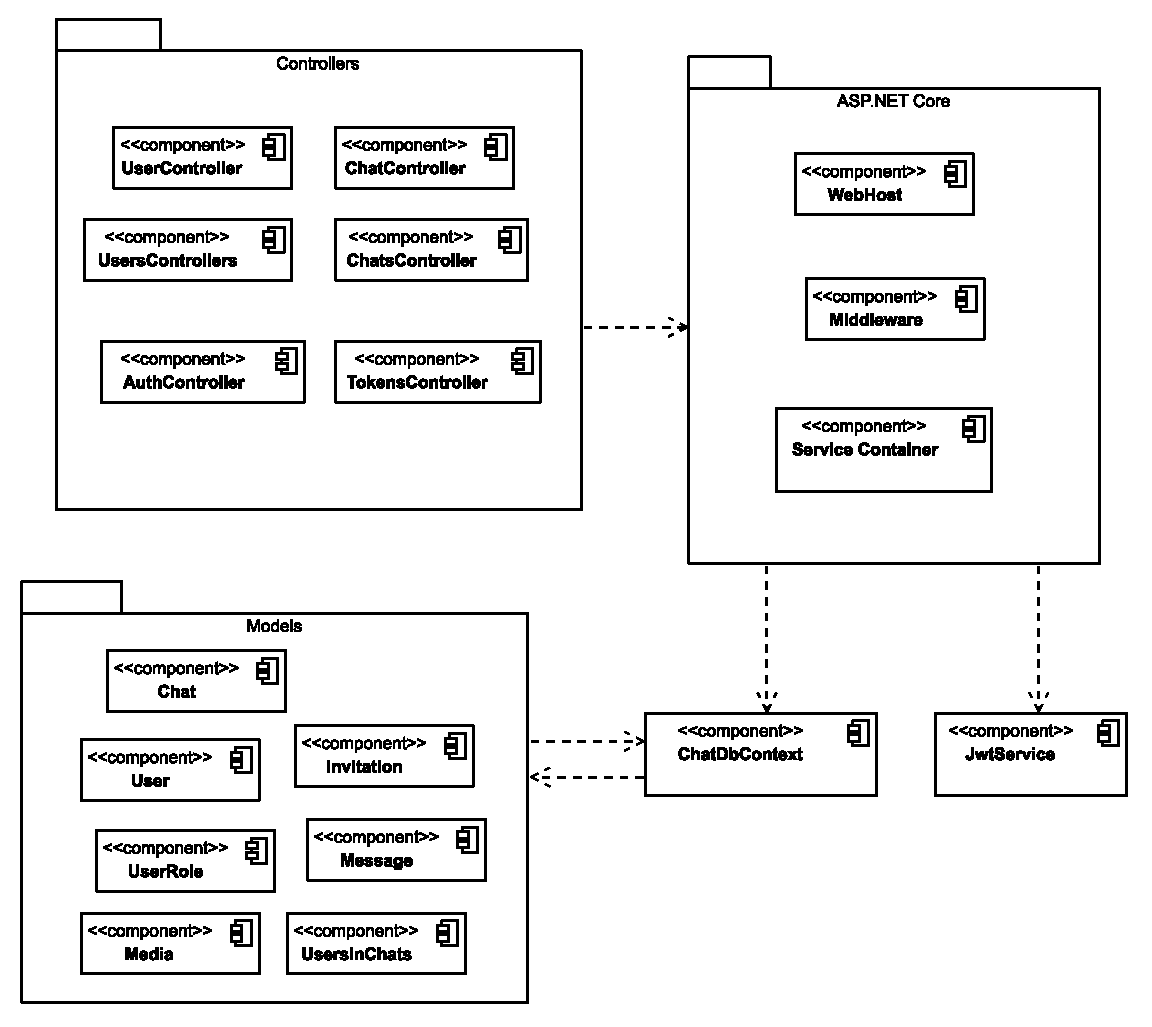
\includegraphics[width=1\linewidth]{components}}
\caption{Диаграмма компонентов}
\label{components:image}
\end{figure}

Программная система включает в себя:
\begin{enumerate}
		\item Клиентская часть: это веб-приложение, разработанное с использованием React-фреймворка Next.js. Она предоставляет пользовательский интерфейс для взаимодействия с приложением чата. Клиентская часть отображает данные, отправленные и полученные от сервера, и обрабатывает пользовательские действия, такие как отправка сообщений и управление чатами.
			
		\item Сервис авторизации: это компонент, ответственный за регистрацию пользователей и управление процессами авторизации и аутентификации в приложении. 
		
		\item Основное приложение: это серверная часть приложения, на котором работает чат. Она обрабатывает запросы от клиентской части, обеспечивает функциональность чата, такую как отправка и получение сообщений, управление пользователями и чатами, и поддерживает взаимодействие с базой данных.
		
		\item База данных: это сервер, на котором развернута PostgreSQL, отвечающая за хранение и управление данными приложения. PostgreSQL используется для хранения пользовательских аккаунтов, сообщений чата, информации о чатах и других необходимых данных. Он обеспечивает надежное хранение и управление данными, а также поддерживает выполнение сложных запросов и транзакций\cite{db}.
\end{enumerate}

\subsection{Модель данных}

На рисунке \ref{data_model:image} в виде UML-диаграммы классов представлена модель данных приложения.

Данный вид диаграмм моделирует статическую структуру системы, отображая классы, их свойства, методы и взаимоотношения между ними. Основная цель диаграммы классов заключается в представлении основных элементов системы и их взаимосвязей, что помогает разработчикам понять структуру и логику системы. Классы представлены в виде прямоугольников, разделенных на три секции: верхняя содержит имя класса, средняя – атрибуты (свойства), а нижняя – операции (методы).

Связи между классами показываются с помощью линий, которые могут быть аннотированы, чтобы указать тип отношения, например ассоциацию, агрегацию, композицию или наследование. Ассоциации показывают базовые связи между классами, агрегации указывают на отношения "часть-целое", композиции – на более сильные связи, где компоненты не могут существовать без целого, а наследование показывает иерархические отношения между классами, где один класс является расширением другого.

Диаграмма классов помогает в проектировании и документировании объектно-ориентированных систем, обеспечивая четкое представление о том, какие классы существуют в системе, какие атрибуты и методы они имеют, и как они взаимодействуют друг с другом.

\begin{landscape}
	\begin{figure}[ht]
		\center{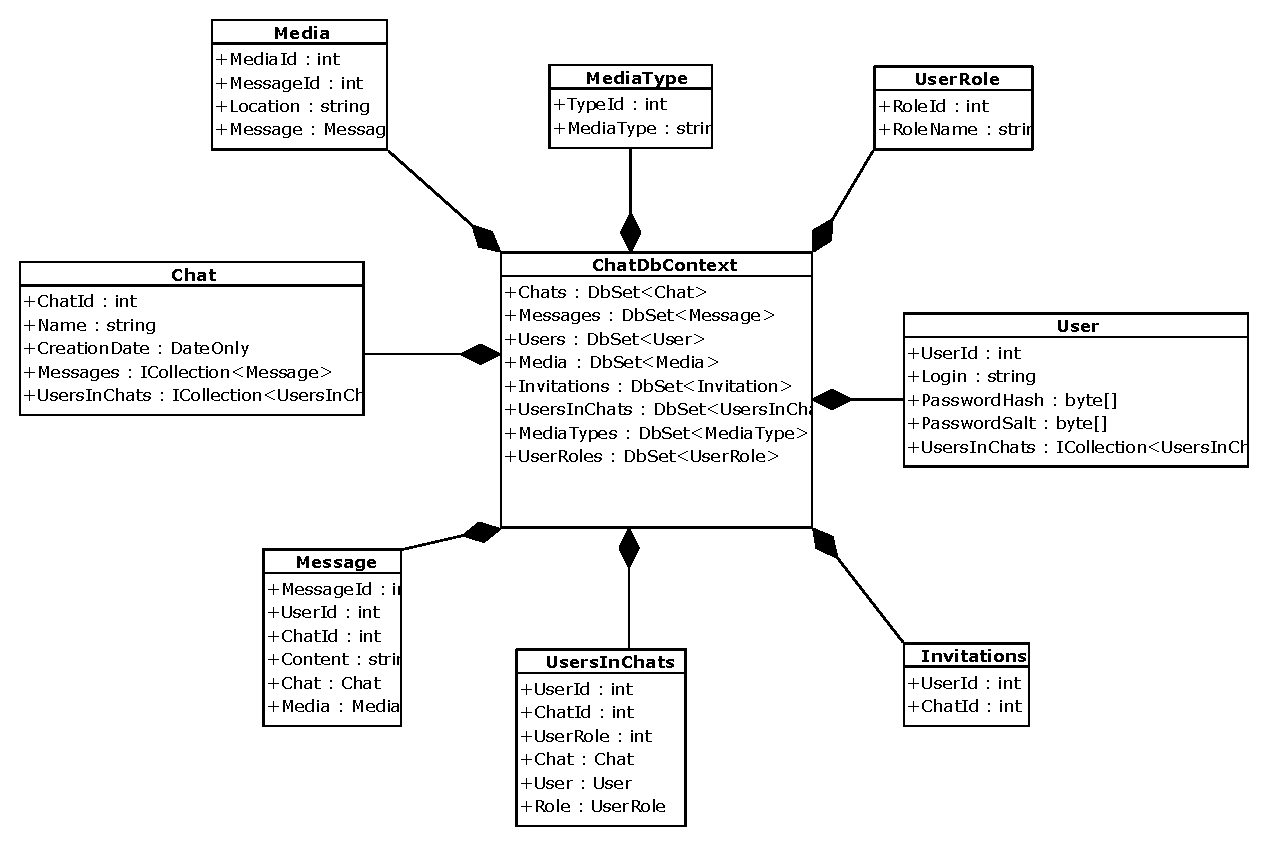
\includegraphics[scale=1.10]{data_model}}
		\caption{Диаграмма классов модели данных}
		\label{data_model:image}
	\end{figure}
\end{landscape}

\begin{itemize}
	\item ChatDbContext - класс, обеспечивающий связь моделей и БД чс Entity Framework. Также описывает правила созания объеков моделей из таблиц БД;
	\item Chat - модель, представляющая собой отображение данных чата;
	\item Media - модель, представляющая собой отображение медиа-файла;
	\item MediaType - модель, представляющая собой отображение типа медиа-файла;
	\item Invitation - модель, представляющая собой отображение приглашения в чат;
	\item Message - модель, представляющая собой отображение данных сообщения;
	\item User - модель, представляющая собой отображение данных пользователя;
	\item UserRole - модель, представляющая собой отображение данных типа роли пользователя;
	\item UsersInChats - модель, представляющая собой отображение данных связи пользователей с их чатами.
\end{itemize}

\subsection{Контроллеры}

На рисунке \ref{controllers:image} представлена диаграмма классов-контроллеров и сервисов, необходимых для их работы.

\begin{landscape}
	\begin{figure}[ht]
		\center{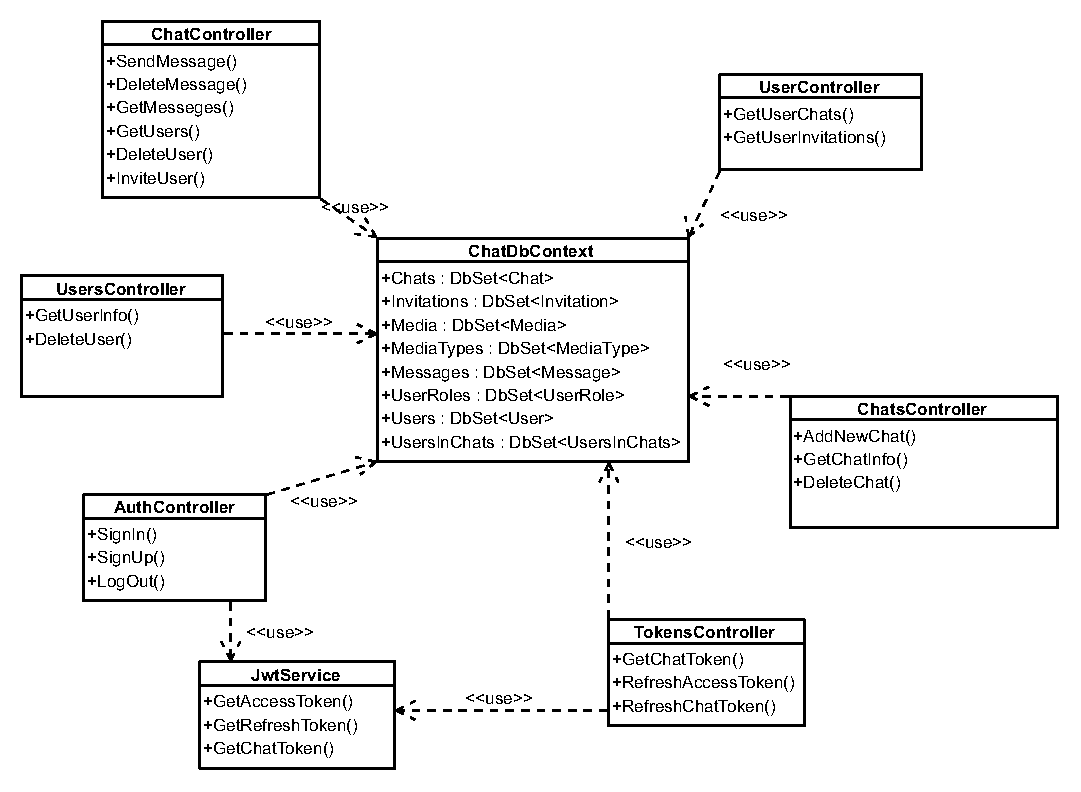
\includegraphics[scale=1.10]{cd_controllers}}
		\caption{Диаграмма классов-контроллеров}
		\label{controllers:image}
	\end{figure}
\end{landscape}

Спецификация диаграммы классов-контроллеров:
\begin{itemize}
	\item ChatDbContext - класс, обеспечивающий связь моделей приложения с фреймворком Entity Framework и предоставляющий доступ контроллерам к данным БД\cite{ef};
	\item JwtService.cs - класс, предоставляющий методы работы с JWT-токенами;
	\item ChatController.cs - класс, предосталяющий методы для работы с конкретным чатом;
	\item UserController.cs - класс, предоставляющий методы для работы с конкретным пользователем приложения;
	\item ChatsController.cs - класс, предоставляющий методы для работы со всеми чатами;
	\item UsersController.cs - класс, предоставляющий методы для работы со всеми пользователями приложения;
	\item AuthController.cs - класс, предоставляющий методы для аутентификации и регистрации пользователей приложения;
	\item TokensController.cs - класс, предоставляющий методы для полуения и обновления токенов.
\end{itemize}

\subsubsection{Представления}

В фреймворке Next.js структура приложения представлена набором страниц, которые в свою очередь состоят из React-компонентов. Компоненты React представляют собой совокупность HTML-подобной разметки и кода JavaScript (TypeScript) для управления состоянием компонента и загрузкой необходимых для отображения данных\cite{nextjs}.

Разрабатываемое прилложение будет содержать следующие страницы:
\begin{itemize}
	\item signup.tsx является представлением для регистрации в приложении;
	\item signin.tsx является представлением для входа в приложение;
	\item main.tsx (включает в себя комоненты AppNavigation, ChatMenu, ChatRoom, Messages, Modal) является основным представлением приложения. Отображает навигацию по приложению и сам чат;
	\item user.tsx представление личного кабинета пользователя для управления персональными данными.
\end{itemize}

\subsubsection{Маршруты приложения}

Для обеспечения доступа пользователей к необходимым информационным ресурсам приложения, разработана карта маршрутов приложения. Описание маршрутов приведено ниже.

POST /Auth/signup - маршрут, предназначенный для регистрации пользователей в приложении. В теле запроса принимает логин и пароль регистрируемого пользователя.

POST /Auth/signin - маршрут, предназначенный для входа пользователей в приложении. В теле запроса принимает логин и пароль пользователя.

GET /Tokens/chat-token - маршрут, предназначенный для выдачи токенов чатов.

GET /Tokens/refresh-chat-token - маршрут, предназначенный для обновления токенов чатов.

GET /Tokens/refresh-access-token - маршрут, предназначенный для обновления токенов доступа.

POST /Chat/send-message - маршрут, предназначенный для отправки сообщений в чате. В теле запроса принимает текст сообщения.

DELETE /Chat/delete-message - маршрут, предназначенный для удаления сообщений из чата. В теле запроса принимает идентификатор удаляемого сообщения.

GET /Chat/messages - маршрут, предназначенный для получения сообщений чата.

GET /Chat/users - маршрут, предназначенный для получения пользователей чата.

POST /Chat/invite - маршрут, предназначенный для приглашения новых пользователей в чат.

DELETE /Chat/delete-user - маршрут, предназначенный для удаления пользователей из чата. В теле запроса принимает идентификатор удаляемого пользователя.

POST /Chats - маршрут, предназначенный для создания нового чата. В теле запроса принимает информацию для создания нового чата.

DELETE /Chats - маршрут, предназначанный для удаления чата. В теле запроса принимает идентификатор удаляемого чата.

GET /User/chats - маршрут, предназначенный для получения чатов, в которых состоит пользователь.

GET /User/invitations - маршрут, предназначенный для получения приглашений пользователя в чаты.

GET /Users - маршрут, предназначенный для полученя информации о конкретном пользователе. В теле запроса принимает идентификатор пользователя, информацию о котором необходимо получить.

DELETE /Users - маршрут, предназначенный для удаления пользователя. В теле запроса принимает идентификатор удаляемого пользователя.

На рисунке \ref{routes:image} представлена схема маршрутов приложения.

\begin{landscape}
	\begin{figure}[ht]
		\center{\includegraphics[width=1\linewidth]{routes}}
		\caption{Маршруты приложения}
		\label{routes:image}
	\end{figure}
\end{landscape}

\subsubsection{Проект данных разрабатываемой системы}

Для организации данных, используемых в разрабатываемой системе, была выбрана реляционная БД PostgreSQL. 

PostgreSQL — это объектно-реляционная система управления базами данных с открытым исходным кодом. Она отличается высокой производительностью, надежностью и масштабируемостью. PostgreSQL поддерживает стандарт SQL и предлагает множество дополнительных возможностей, таких как полнотекстовый поиск, индексирование, транзакции с поддержкой ACID, расширения для различных типов данных, включая JSON и XML. Система активно развивается и поддерживается сообществом, что обеспечивает её актуальность и адаптацию к современным требованиям. PostgreSQL подходит для различных типов приложений, от небольших веб-приложений до крупных корпоративных систем.

Был выбран подход Database First\cite{ef}, т. е. сначала разрабатывается схема БД, а затем на ее основе средствами Entity Framework генерируются модели приложения.

Схема БД состоит из следующих таблиц:
\begin{itemize}
	\item chats - чаты;
	\item invitations - приглашения пользователей в чаты;
	\item messages - сообщения в чатах;
	\item media - загруженные файлы;
	\item media\_type - тип загруженного файла;
	\item user - пользователи приложения;
	\item user\_role - роли пользователей;
	\item users\_in\_chats - таблица связи пользователей и чатов, в которых они состоят. 
\end{itemize}

ER-диаграмма БД представлена на рисунке \ref{erd:image}.

\begin{figure}[H]
	\center{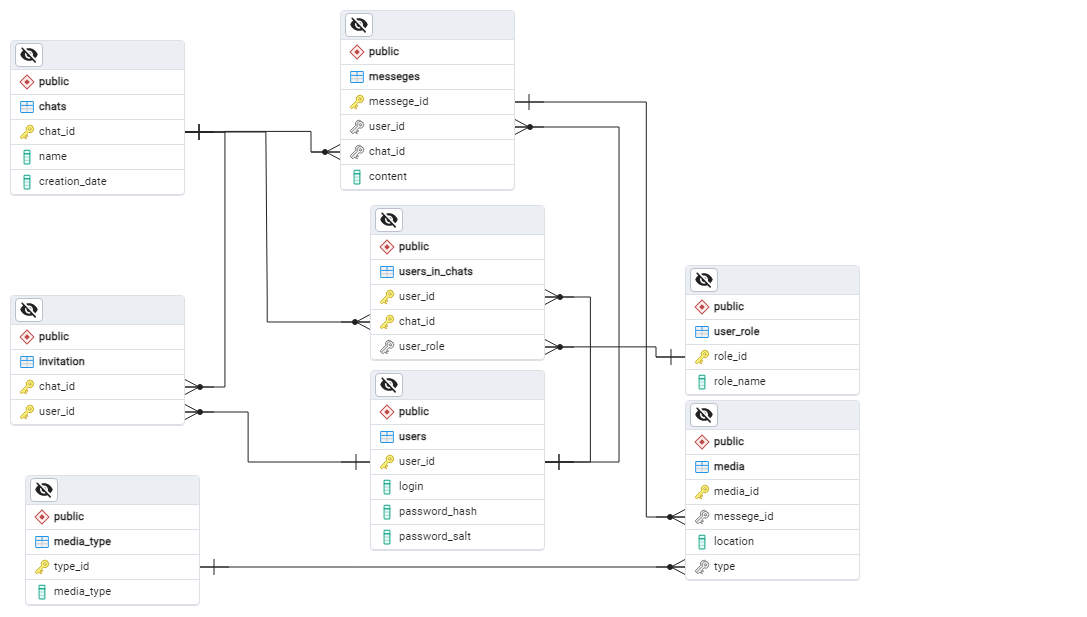
\includegraphics[width=1\linewidth]{erd}}
	\caption{ER-диаграмма базы данных}
	\label{erd:image}
\end{figure}

В таблице \ref{chats:table} представлены атрибуты сущности "<Чат">.

\begin{xltabular}{\textwidth}{|X|p{2.5cm}|p{3cm}|>{\setlength{\baselineskip}{0.7\baselineskip}}p{4.83cm}|}
	\caption{Описание полей таблицы "chats"\label{chats:table}} \hline
	\centrow Поле & \centrow Тип & \centrow Обязательное & \centrow Описание \\ \hline
	\centrow 1 & \centrow 2 & \centrow 3 & \centrow 4\\ \hline
	\endfirsthead
	\continuecaption{Продолжение таблицы \ref{chats:table}} \hline
	\centrow 1 & \centrow 2 & \centrow 3 & \centrow 4\\ \hline
	\finishhead
	chat\_id & integer & да & Идентификатор чата (автоматический) \\ \hline
	name & character varying(128) & да & Название чата \\ \hline
	creation\_date & date & да & Дата создания чата \\ \hline
\end{xltabular}

В таблице \ref{invitations:table} представлены атрибуты сущности "<Приглашение">.

\begin{xltabular}{\textwidth}{|X|p{2.5cm}|p{3cm}|>{\setlength{\baselineskip}{0.7\baselineskip}}p{4.83cm}|}
	\caption{Описание полей таблицы "invitations"\label{invitations:table}} \hline
	\centrow Поле & \centrow Тип &  \centrow Обязательное & \centrow Описание \\ \hline
	\centrow 1 & \centrow 2 & \centrow 3 & \centrow 4\\ \hline
	\endfirsthead
	\continuecaption{Продолжение таблицы \ref{invitations:table}} \centrow 1 & \centrow 2 & \centrow 3 & \centrow 4\\ \hline
	\finishhead
	chat\_id & integer & да & Идентификатор чата \\ \hline
	user\_id & integer & да & Идентификатор приглашемого пользователя \\ \hline
\end{xltabular}

В таблице \ref{messages:table} представлены атрибуты сущности "<Сообщение">.

\begin{xltabular}{\textwidth}{|X|p{2.5cm}|p{3cm}|>{\setlength{\baselineskip}{0.7\baselineskip}}p{4.83cm}|}
	\caption{Описание полей таблицы "messages"\label{messages:table}} \hline
	Поле & Тип & Обязательное & Описание \\ \hline
	\centrow 1 & \centrow 2 & \centrow 3 & \centrow 4\\ \hline
	\endfirsthead
	\continuecaption{Продолжение таблицы \ref{messages:table}} \hline
	\centrow 1 & \centrow 2 & \centrow 3 & \centrow 4\\ \hline
	\finishhead
	message\_id & integer & да & Идентификатор сообщения (автоматический) \\ \hline
	user\_id & integer & нет & Идентификатор пользователя (если есть) \\ \hline
	chat\_id & integer & да & Идентификатор чата \\ \hline
	content & text & нет & Содержание сообщения \\ \hline
\end{xltabular}

В таблице \ref{media:table} представлены атрибуты сущности "<Медиа">.

\begin{xltabular}{\textwidth}{|X|p{2.5cm}|p{3cm}|>{\setlength{\baselineskip}{0.7\baselineskip}}p{4.83cm}|}
	\caption{Описание полей таблицы "media"\label{media:table}} \hline
	Поле & Тип & Обязательное & Описание \\ \hline
	\centrow 1 & \centrow 2 & \centrow 3 & \centrow 4\\ \hline
	\endfirsthead
	\continuecaption{Продолжение таблицы \ref{media:table}} \hline
	\centrow 1 & \centrow 2 & \centrow 3 & \centrow 4\\ \hline
	\finishhead
	media\_id & serial & да & Идентификатор медиа (автоматический) \\ \hline
	location & text & да & Местоположение медиа \\ \hline
	type & integer & да & Тип медиа \\ \hline
\end{xltabular}

В таблице \ref{media_type:table} представлены атрибуты сущности "<Тип медиа">.

\begin{xltabular}{\textwidth}{|X|p{2.5cm}|p{3cm}|>{\setlength{\baselineskip}{0.7\baselineskip}}p{4.83cm}|}
	\caption{Описание полей таблицы "media\_type"\label{media_type:table}} \hline
	\centrow Поле & \centrow Тип & \centrow Обязательное & \centrow Описание \\ \hline
	\centrow 1 & \centrow 2 & \centrow 3 & \centrow 4\\ \hline
	\endfirsthead
	\continuecaption{Продолжение таблицы \ref{media_type:table}} \centrow 1 & \centrow 2 & \centrow 3 & \centrow 4\\ \hline
	\finishhead
	type\_id & int & да & Идентификатор типа медиа \\ \hline
	media\_type & character varying(20) & да & Тип медиа \\ \hline
\end{xltabular}

В таблице \ref{users:table} представлены атрибуты сущности "<Пользователь">.

\begin{xltabular}{\textwidth}{|X|p{2.5cm}|p{3cm}|>{\setlength{\baselineskip}{0.7\baselineskip}}p{4.83cm}|}
	\caption{Описание полей таблицы "users"\label{users:table}} \hline
	\centrow Поле & \centrow Тип & \centrow Обязательное & \centrow Описание \\ \hline
	\centrow 1 & \centrow 2 & \centrow 3 & \centrow 4\\ \hline
	\endfirsthead
	\continuecaption{Продолжение таблицы \ref{users:table}} \hline
	\centrow 1 & \centrow 2 & \centrow 3 & \centrow 4\\ \hline
	\finishhead
	user\_id & integer & да & Идентификатор пользователя (автоматический) \\ \hline
	login & character varying(64) & да & Логин пользователя \\ \hline
	password\_hash & bytea & да & Хэш пароля пользователя \\ \hline
	password\_salt & bytea & да & Соль пароля пользователя \\ \hline
\end{xltabular}

В таблице \ref{user_role:table} представлены атрибуты сущности "<Роль пользователя">.

\begin{xltabular}{\textwidth}{|X|p{2.5cm}|p{3cm}|>{\setlength{\baselineskip}{0.7\baselineskip}}p{4.83cm}|}
	\caption{Описание полей таблицы "user\_role"\label{user_role:table}} \hline
	\centrow Поле & \centrow Тип & \centrow Обязательное & \centrow Описание \\ \hline
	\centrow 1 & \centrow 2 & \centrow 3 & \centrow 4\\ \hline
	\endfirsthead
	\continuecaption{Продолжение таблицы \ref{user_role:table}} \\ \hline
	\centrow 1 & \centrow 2 & \centrow 3 & \centrow 4\\ \hline
	\finishhead
	role\_id & integer & да & Идентификатор роли пользователя \\ \hline
	role\_name & character varying(15) & да & Наименование роли пользователя \\ \hline
\end{xltabular}

В таблице \ref{users_in_chats:table} представлены атрибуты сущности "<Пользователи в чатах">.

\begin{xltabular}{\textwidth}{|X|p{2.5cm}|p{3cm}|>{\setlength{\baselineskip}{0.7\baselineskip}}p{4.83cm}|}
	\caption{Описание полей таблицы "users\_in\_chats"\label{users_in_chats:table}} \hline
	\centrow Поле & \centrow Тип & \centrow Обязательное & \centrow Описание \\ \hline
	\centrow 1 & \centrow 2 & \centrow 3 & \centrow 4\\ \hline
	\endfirsthead
	\continuecaption{Продолжение таблицы \ref{users_in_chats:table}} \hline \centrow 1 & \centrow 2 & \centrow 3 & \centrow 4\\ \hline
	\endhead
	Поле & Тип & Обязательное & Описание \\ \hline
	\finishhead
	user\_id & integer & да & Идентификатор пользователя \\ \hline
	chat\_id & integer & да & Идентификатор чата \\ \hline
	user\_role & integer & да & Роль пользователя в чате \\ \hline
\end{xltabular}

\subsection{Проектирование пользоватеьского интерфейса}

Учитывая требования к пользовательскому интерфейсу, сформированные в пункте технического задания, был разработан интерфейс программной системы. 

Ниже приведены макеты интерфейса десктопной версии приложения. В мобильной версии компоненты такие же как и в десктопной, но размещены с учетом удобства использования на портативных устройствах.

На рисунках ниже компоненты интерфейса пронумированы.

На рисунке \ref{signup_maket:image} представлен макет страницы регистрации. Эта страница содержит следующие компоненты:
\begin{itemize}
	\item поле для ввода логина;
	\item поле для ввода пароля;
	\item поле для ввода подтверждения пароля;
	\item кнопка "<Зарегистрироваться">;
	\item кнопка "<Войти">.
\end{itemize}

\begin{figure}[H]
	\center{
\includegraphics[width=1\linewidth]{signup_maket}}
	\caption{Макет страницы регистрации}
	\label{signup_maket:image}
\end{figure}

На рисунке \ref{signin_maket:image} представлен макет страницы входа. Эта страница содержит следующие компоненты:
\begin{itemize}
	\item поле для ввода логина;
	\item поле для ввода пароля;
	\item кнопка "<Войти">;
	\item сссылка на страницу регистрации.
\end{itemize}

\begin{figure}[H]
	\center{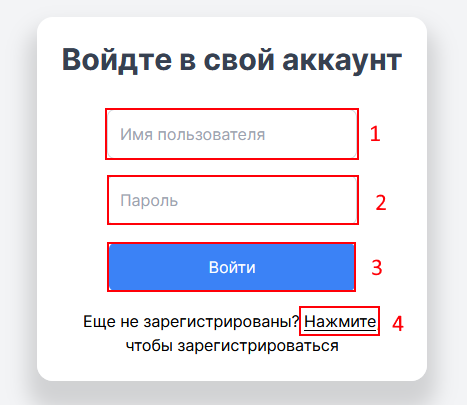
\includegraphics[width=1\linewidth]{signin_maket}}
	\caption{Макет страницы входа}
	\label{signin_maket:image}
\end{figure}

На рисунке \ref{main_maket:image} представлен макет страницы входа. Эта страница содержит следующие компоненты:
\begin{itemize}
	\item список чатов;
	\item кнопка перехода на страницу пользователя;
	\item кнопка создания чата;
	\item кнопка поиска по чатам;
	\item вкладка "<Чаты">;
	\item вкладка "<Приглашения">;
	\item список сообщений чата;
	\item кнопка меню настроек чата;
	\item кнопка отпраки файла;
	\item поле ввода сообщения;
	\item кнопка отправки сообщения.
\end{itemize}

\begin{figure}[H]
	\center{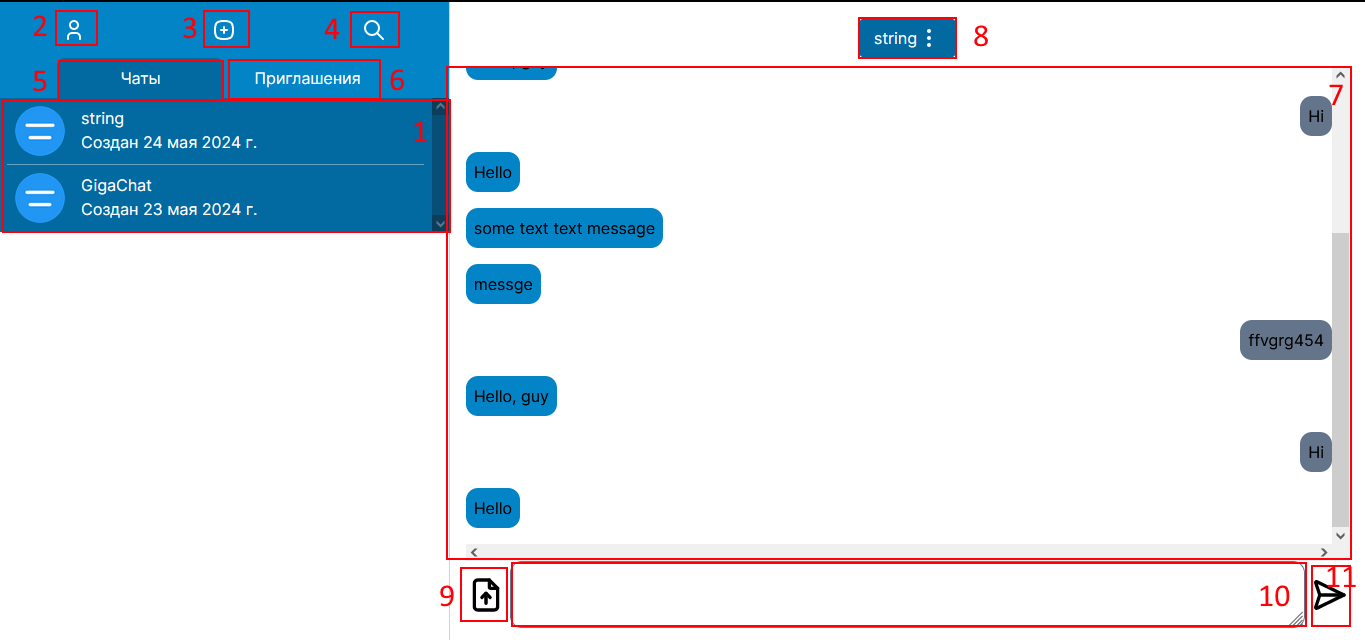
\includegraphics[width=1\linewidth]{main_maket}}
	\caption{Макет основной страницы}
	\label{main_maket:image}
\end{figure}

На рисунке \ref{cabinet_maket:image} представлен макет страницы входа. Эта страница содержит следующие компоненты:
\begin{itemize}
	\item поле для изменения логина пользователя;
	\item кнопка для подтверждения изменения логина;
	\item поле для изменения пароля пользователя;
	\item поле для подтверждения нового пароля;
	\item кнопка для подтверждения изменения пароля.
\end{itemize}

\begin{figure}[H]
	\center{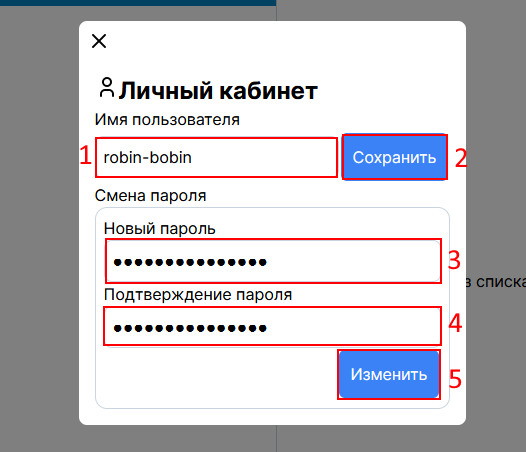
\includegraphics[width=1\linewidth]{cabinet_maket}}
	\caption{Макет кабинет пользователя}
	\label{cabinet_maket:image}
\end{figure}
\ifПрактика{}\else{
   \section{Рабочий проект}
\subsection{Описание компонентов и классов программы}
\subsubsection{Описание классов сервиса аутентификации}
\paragraph{Описание класса AuthController}

Описание полей и методов класса AuthController представлено в таблицах \ref{classAuthFields:table} и \ref{classAuthMethods:table} соответственно.

\renewcommand{\arraystretch}{0.8} % уменьшение расстояний до сетки таблицы
\begin{xltabular}{\textwidth}{|X|p{2.5cm}|>{\setlength{\baselineskip}{0.7\baselineskip}}p{4.83cm}|>{\setlength{\baselineskip}{0.7\baselineskip}}p{4.85cm}|}
	\caption{Описание полей класса AuthController}\label{classAuthFields:table}
	\hline \centrow \setlength{\baselineskip}{0.7\baselineskip} Название поля & \centrow \setlength{\baselineskip}{0.7\baselineskip} Область видимости & \centrow Тип данных & \centrow Описание \\
	\hline \centrow 1 & \centrow 2 & \centrow 3 & \centrow 4\\ \hline
	\endfirsthead
	\continuecaption{Продолжение таблицы \ref{classAuthFields:table}}
	\hline \centrow 1 & \centrow 2 & \centrow 3 & \centrow 4\\ \hline
	\finishhead
	dbContext & private & ChatDbContext & Контекст базы данных приложения\\
	\hline jwtService & private & JwtService & Сервис, отвечающий за работу с jwt-токенами \\
\end{xltabular}
\renewcommand{\arraystretch}{1.0}

\begin{xltabular}{\textwidth}{|X|p{2.5cm}|>{\setlength{\baselineskip}{0.7\baselineskip}}p{4.83cm}|}
	\caption{Описание методов класса AuthController}\label{classAuthMethods:table}
	\hline \centrow Название поля & \centrow Область видимости & \centrow Описание \\ \hline \centrow 1 & \centrow 2 & \centrow 3\\
	\hline 
	\endfirsthead
	\continuecaption{Продолжение таблицы \ref{classAuthMethods:table}}
	\hline \centrow 1 & \centrow 2 & \centrow 3 \\ \hline
	\hline \centrow Название поля & \centrow Область видимости & \centrow Описание \\ \hline
	\endhead
	SignUp & public & Действие контроллера, отвечающее за регистрацию пользователей \\ \hline
	SignIn & public & Действие контроллера, отвечающее за авторизацию пользователей \\ \hline
\end{xltabular}

\renewcommand{\arraystretch}{1.0}

\paragraph{Описание класса TokensController}

Описание полей и методов класса TokensController представлено в таблицах \ref{classTokensFields:table} и \ref{classTokensMethods:table} соответственно.

\renewcommand{\arraystretch}{0.8} % уменьшение расстояний до сетки таблицы
\begin{xltabular}{\textwidth}{|X|p{2.5cm}|>{\setlength{\baselineskip}{0.7\baselineskip}}p{4.83cm}|>{\setlength{\baselineskip}{0.7\baselineskip}}p{4.85cm}|}
	\caption{Описание полей класса AuthController}\label{classTokensFields:table}
	\hline \centrow \setlength{\baselineskip}{0.7\baselineskip} Название поля & \centrow \setlength{\baselineskip}{0.7\baselineskip} Область видимости & \centrow Тип данных & \centrow Описание \\
	\hline \centrow 1 & \centrow 2 & \centrow 3 & \centrow 4\\ \hline
	\endfirsthead
	\continuecaption{Продолжение таблицы \ref{classTokensFields:table}}
	\hline \centrow 1 & \centrow 2 & \centrow 3 & \centrow 4\\ \hline
	\finishhead
	dbContext & private & ChatDbContext & Контекст базы данных приложения\\
	\hline jwtService & private & JwtService & Сервис, отвечающий за работу с jwt-токенами \\
\end{xltabular}
\renewcommand{\arraystretch}{1.0}

\begin{xltabular}{\textwidth}{|X|p{2.5cm}|>{\setlength{\baselineskip}{0.7\baselineskip}}p{4.83cm}|}
	\caption{Описание методов класса AuthController}\label{classTokensMethods:table}
	\hline \centrow Название поля & \centrow Область видимости & \centrow Описание \\ \hline \centrow 1 & \centrow 2 & \centrow 3\\
	\hline 
	\endfirsthead
	\continuecaption{Продолжение таблицы \ref{classTokensMethods:table}}
	\hline \centrow 1 & \centrow 2 & \centrow 3 \\ \hline
	\hline \centrow Название поля & \centrow Область видимости & \centrow Описание \\ \hline
	\endhead
	GetChatToken & public & Действие контроллера, отвечающее за выдачу токенов конкретного чата \\ \hline
	RefreshAccessToken & public & Действие контроллера, отвечающее за обновление токена доступа \\ \hline
	RefreshChatToken & public & Действие контроллера, отвечающее за обновление токенов чатов \\ \hline
\end{xltabular}

\renewcommand{\arraystretch}{1.0}

\paragraph{Описание класса JwtService}

Описание полей и методов класса JwtService представлено в таблицах \ref{classJwtFields:table} и \ref{classJwtMethods:table} соответственно.

\renewcommand{\arraystretch}{0.8} % уменьшение расстояний до сетки таблицы
\begin{xltabular}{\textwidth}{|X|p{2.5cm}|>{\setlength{\baselineskip}{0.7\baselineskip}}p{4.83cm}|>{\setlength{\baselineskip}{0.7\baselineskip}}p{4.85cm}|}
	\caption{Описание полей класса JwtService}\label{classJwtFields:table}
	\hline \centrow \setlength{\baselineskip}{0.7\baselineskip} Название поля & \centrow \setlength{\baselineskip}{0.7\baselineskip} Область видимости & \centrow Тип данных & \centrow Описание \\
	\hline \centrow 1 & \centrow 2 & \centrow 3 & \centrow 4\\ \hline
	\endfirsthead
	\continuecaption{Продолжение таблицы \ref{classJwtFields:table}}
	\hline \centrow 1 & \centrow 2 & \centrow 3 & \centrow 4\\ \hline
	\finishhead
	configuration & private & IConfiguration & Данное поле обеспечивает к конфигурации приложения\\
\end{xltabular}
\renewcommand{\arraystretch}{1.0}

\begin{xltabular}{\textwidth}{|X|p{2.5cm}|>{\setlength{\baselineskip}{0.7\baselineskip}}p{4.83cm}|}
	\caption{Описание методов класса JwtService}\label{classJwtMethods:table}
	\hline \centrow Название поля & \centrow Область видимости & \centrow Описание \\ \hline \centrow 1 & \centrow 2 & \centrow 3\\
	\hline 
	\endfirsthead
	\continuecaption{Продолжение таблицы \ref{classJwtMethods:table}}
	\hline \centrow 1 & \centrow 2 & \centrow 3 \\ \hline
	\hline \centrow Название поля & \centrow Область видимости & \centrow Описание \\ \hline
	\endhead
	GetAccessToken & public & Метод, отвечающий за генерацию токенов доступа \\ \hline
	GetRefreshToken & public & Метод, отвечающий за генерацию токенов обновления \\ \hline
	GetChatToken & public & Метод, отвечающий за генерацию токенов чатов \\ \hline
\end{xltabular}

\renewcommand{\arraystretch}{1.0}

\subsubsection{Описание классов приложения}

\paragraph{Описание класса ChatController}

Описание полей и методов класса ChatController представлено в таблицах \ref{classChatFields:table} и \ref{classChatMethods:table} соответственно.

\renewcommand{\arraystretch}{0.8} % уменьшение расстояний до сетки таблицы
\begin{xltabular}{\textwidth}{|X|p{2.5cm}|>{\setlength{\baselineskip}{0.7\baselineskip}}p{4.83cm}|>{\setlength{\baselineskip}{0.7\baselineskip}}p{4.85cm}|}
	\caption{Описание полей класса ChatController}\label{classChatFields:table}
	\hline \centrow \setlength{\baselineskip}{0.7\baselineskip} Название поля & \centrow \setlength{\baselineskip}{0.7\baselineskip} Область видимости & \centrow Тип данных & \centrow Описание \\
	\hline \centrow 1 & \centrow 2 & \centrow 3 & \centrow 4\\ \hline
	\endfirsthead
	\continuecaption{Продолжение таблицы \ref{classChatFields:table}}
	\hline \centrow 1 & \centrow 2 & \centrow 3 & \centrow 4\\ \hline
	\finishhead
	dbContext & private & ChatDbContext & Контекст базы данных приложения\\
	\hline hubContext & private & IHubContext<ChatHub> & Контекст хаба чатов, для возможности рассылки обновлений пользователям чата в реальном времени \\
\end{xltabular}
\renewcommand{\arraystretch}{1.0}

\begin{xltabular}{\textwidth}{|X|p{2.5cm}|>{\setlength{\baselineskip}{0.7\baselineskip}}p{4.83cm}|}
	\caption{Описание методов класса AuthController}\label{classChatMethods:table}
	\hline \centrow Название поля & \centrow Область видимости & \centrow Описание \\ \hline \centrow 1 & \centrow 2 & \centrow 3\\
	\hline 
	\endfirsthead
	\continuecaption{Продолжение таблицы \ref{classChatMethods:table}}
	\hline \centrow 1 & \centrow 2 & \centrow 3 \\ \hline
	\hline \centrow Название метода & \centrow Область видимости & \centrow Описание \\ \hline
	\endhead
	SendMessage & public & Метод, отвечающий за отправку сообщения в чат \\ \hline
	DeleteMessage & public & Метод, отвечающий за удаление сообщения из чата \\ \hline
	GetMessages & public & Метод, возвращающий все сообщения чата \\ \hline
	GetUsers & public & Метод, возвращающий всех пользователей в чате \\ \hline
	DeleteUser & public & Метод, отвечающий за удаление пользователя из чата \\ \hline
\end{xltabular}

\renewcommand{\arraystretch}{1.0}

\paragraph{Описание класса ChatsController}

Описание полей и методов класса ChastController представлено в таблицах \ref{classChatsFields:table} и \ref{classChatsMethods:table} соответственно.

\renewcommand{\arraystretch}{0.8} % уменьшение расстояний до сетки таблицы
\begin{xltabular}{\textwidth}{|X|p{2.5cm}|>{\setlength{\baselineskip}{0.7\baselineskip}}p{4.83cm}|>{\setlength{\baselineskip}{0.7\baselineskip}}p{4.85cm}|}
	\caption{Описание полей класса ChatsController}\label{classChatsFields:table}
	\hline \centrow \setlength{\baselineskip}{0.7\baselineskip} Название поля & \centrow \setlength{\baselineskip}{0.7\baselineskip} Область видимости & \centrow Тип данных & \centrow Описание \\
	\hline \centrow 1 & \centrow 2 & \centrow 3 & \centrow 4\\ \hline
	\endfirsthead
	\continuecaption{Продолжение таблицы \ref{classChatsFields:table}}
	\hline \centrow 1 & \centrow 2 & \centrow 3 & \centrow 4\\ \hline
	\finishhead
	dbContext & private & ChatDbContext & Контекст базы данных приложения \\
\end{xltabular}
\renewcommand{\arraystretch}{1.0}

\begin{xltabular}{\textwidth}{|X|p{2.5cm}|>{\setlength{\baselineskip}{0.7\baselineskip}}p{4.83cm}|}
	\caption{Описание методов класса ChatsController}\label{classChatsMethods:table}
	\hline \centrow Название поля & \centrow Область видимости & \centrow Описание \\ \hline \centrow 1 & \centrow 2 & \centrow 3\\
	\hline 
	\endfirsthead
	\continuecaption{Продолжение таблицы \ref{classChatsMethods:table}}
	\hline \centrow 1 & \centrow 2 & \centrow 3 \\ \hline
	\hline \centrow Название метода & \centrow Область видимости & \centrow Описание \\ \hline
	\endhead
	AddNewChat & public & Метод, отвечающий за добавление нового чата \\ \hline
	DeleteChat & public & Метод, отвечающий за удаление чата \\ \hline
	UpdateChat & public & Метод, отвечающий за обновлении информации о чате \\ \hline
\end{xltabular}

\renewcommand{\arraystretch}{1.0}

\paragraph{Описание класса UserController}

Описание полей и методов класса UserController представлено в таблицах \ref{classUserFields:table} и \ref{classUserMethods:table} соответственно.

\renewcommand{\arraystretch}{0.8} % уменьшение расстояний до сетки таблицы
\begin{xltabular}{\textwidth}{|X|p{2.5cm}|>{\setlength{\baselineskip}{0.7\baselineskip}}p{4.83cm}|>{\setlength{\baselineskip}{0.7\baselineskip}}p{4.85cm}|}
	\caption{Описание полей класса UserController}\label{classUserFields:table}
	\hline \centrow \setlength{\baselineskip}{0.7\baselineskip} Название поля & \centrow \setlength{\baselineskip}{0.7\baselineskip} Область видимости & \centrow Тип данных & \centrow Описание \\
	\hline \centrow 1 & \centrow 2 & \centrow 3 & \centrow 4\\ \hline
	\endfirsthead
	\continuecaption{Продолжение таблицы \ref{classUserFields:table}}
	\hline \centrow 1 & \centrow 2 & \centrow 3 & \centrow 4\\ \hline
	\finishhead
	dbContext & private & ChatDbContext & Контекст базы данных приложения \\
\end{xltabular}
\renewcommand{\arraystretch}{1.0}

\begin{xltabular}{\textwidth}{|X|p{2.5cm}|>{\setlength{\baselineskip}{0.7\baselineskip}}p{4.83cm}|}
	\caption{Описание методов класса ChatsController}\label{classUserMethods:table}
	\hline \centrow Название поля & \centrow Область видимости & \centrow Описание \\ \hline \centrow 1 & \centrow 2 & \centrow 3\\
	\hline 
	\endfirsthead
	\continuecaption{Продолжение таблицы \ref{classUserMethods:table}}
	\hline \centrow 1 & \centrow 2 & \centrow 3 \\ \hline
	\hline \centrow Название метода & \centrow Область видимости & \centrow Описание \\ \hline
	\endhead
	GetUserChats & public & Метод, отвечающий за получение чатов, в которых состоит пользователь \\ \hline
	GetUserInvitations & public & Метод, отвечающий за получение приглашений пользователя в чаты \\ \hline
\end{xltabular}

\renewcommand{\arraystretch}{1.0}

\paragraph{Описание класса UserController}

Описание полей и методов класса UsersController представлено в таблицах \ref{classUsersFields:table} и \ref{classUsersMethods:table} соответственно.

\renewcommand{\arraystretch}{0.8} % уменьшение расстояний до сетки таблицы
\begin{xltabular}{\textwidth}{|X|p{2.5cm}|>{\setlength{\baselineskip}{0.7\baselineskip}}p{4.83cm}|>{\setlength{\baselineskip}{0.7\baselineskip}}p{4.85cm}|}
	\caption{Описание полей класса UserController}\label{classUsersFields:table}
	\hline \centrow \setlength{\baselineskip}{0.7\baselineskip} Название поля & \centrow \setlength{\baselineskip}{0.7\baselineskip} Область видимости & \centrow Тип данных & \centrow Описание \\
	\hline \centrow 1 & \centrow 2 & \centrow 3 & \centrow 4\\ \hline
	\endfirsthead
	\continuecaption{Продолжение таблицы \ref{classUsersFields:table}}
	\hline \centrow 1 & \centrow 2 & \centrow 3 & \centrow 4\\ \hline
	\finishhead
	dbContext & private & ChatDbContext & Контекст базы данных приложения \\
\end{xltabular}
\renewcommand{\arraystretch}{1.0}

\begin{xltabular}{\textwidth}{|X|p{2.5cm}|>{\setlength{\baselineskip}{0.7\baselineskip}}p{4.83cm}|}
	\caption{Описание методов класса ChatsController}\label{classUsersMethods:table}
	\hline \centrow Название поля & \centrow Область видимости & \centrow Описание \\ \hline \centrow 1 & \centrow 2 & \centrow 3\\
	\hline 
	\endfirsthead
	\continuecaption{Продолжение таблицы \ref{classUsersMethods:table}}
	\hline \centrow 1 & \centrow 2 & \centrow 3 \\ \hline
	\hline \centrow Название метода & \centrow Область видимости & \centrow Описание \\ \hline
	\finishhead
	DeleteUser & public & Метод, отвечающий за удаление пользователя \\ \hline
	UpdateUser & public & Метод, отвечающий за обновление данных пользователя \\ \hline
\end{xltabular}

\renewcommand{\arraystretch}{1.0}

\subsection{Тестирование программной системы}

\subsubsection{Системное тестирование}

Для проверки работоспособности разработанной программной системы было произведено системное тестирование приложения. На нижеприведенных рисунках представлены результаты тестирования системы.

Произведем тестирование функционала регистрации в приложении. Для этого необходимо ввести данные для регистрациии и нажать кнопку "<Зарегистрироваться">. После регистрации пользователь должен быть перенаправлен на основную страницу приложения. Результаты тестирования данного функционала представлены на рисунках \ref{signup_test1:image}-\ref{signup_test3:image}. 

\begin{figure}[H]
	\center{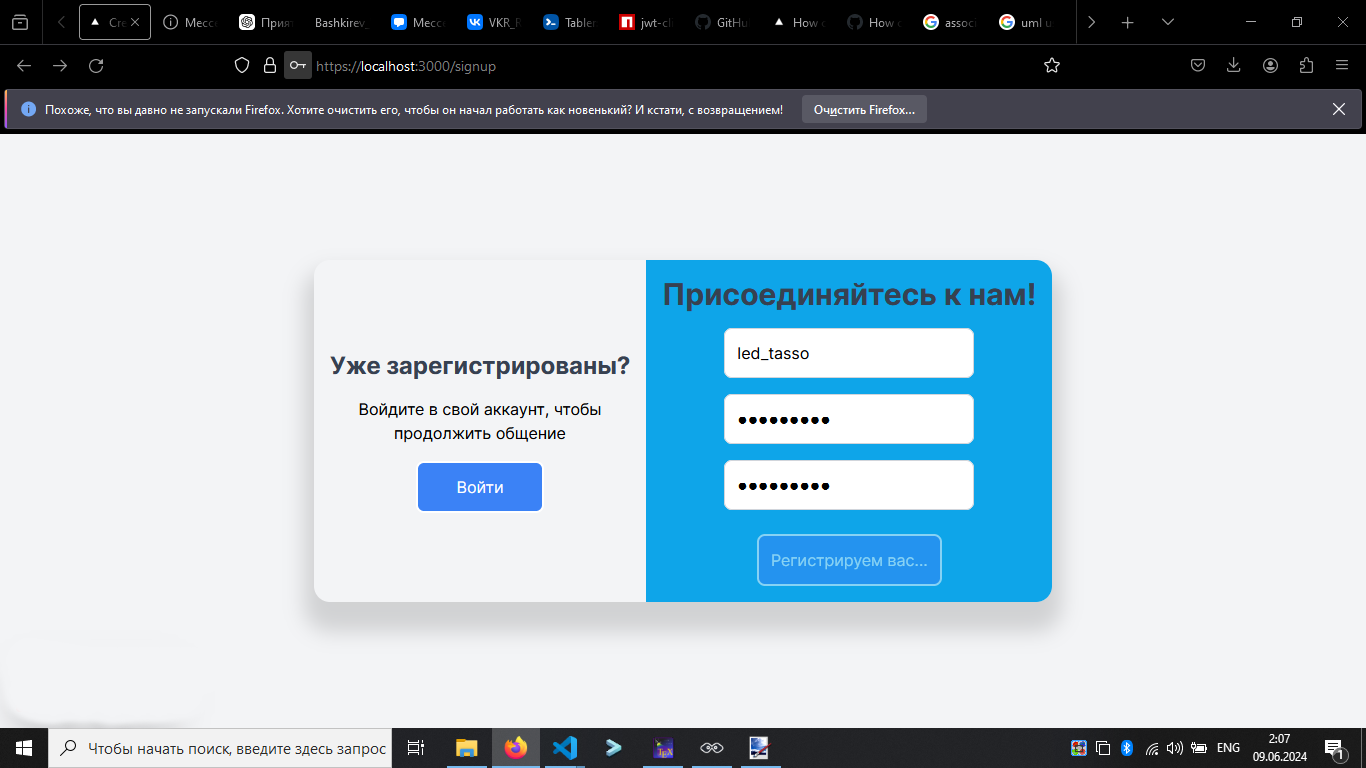
\includegraphics[width=1\linewidth]{signup_test1}}
	\caption{Процесс регистрации пользователя}
	\label{signup_test1:image}
\end{figure}

\begin{figure}[H]
	\center{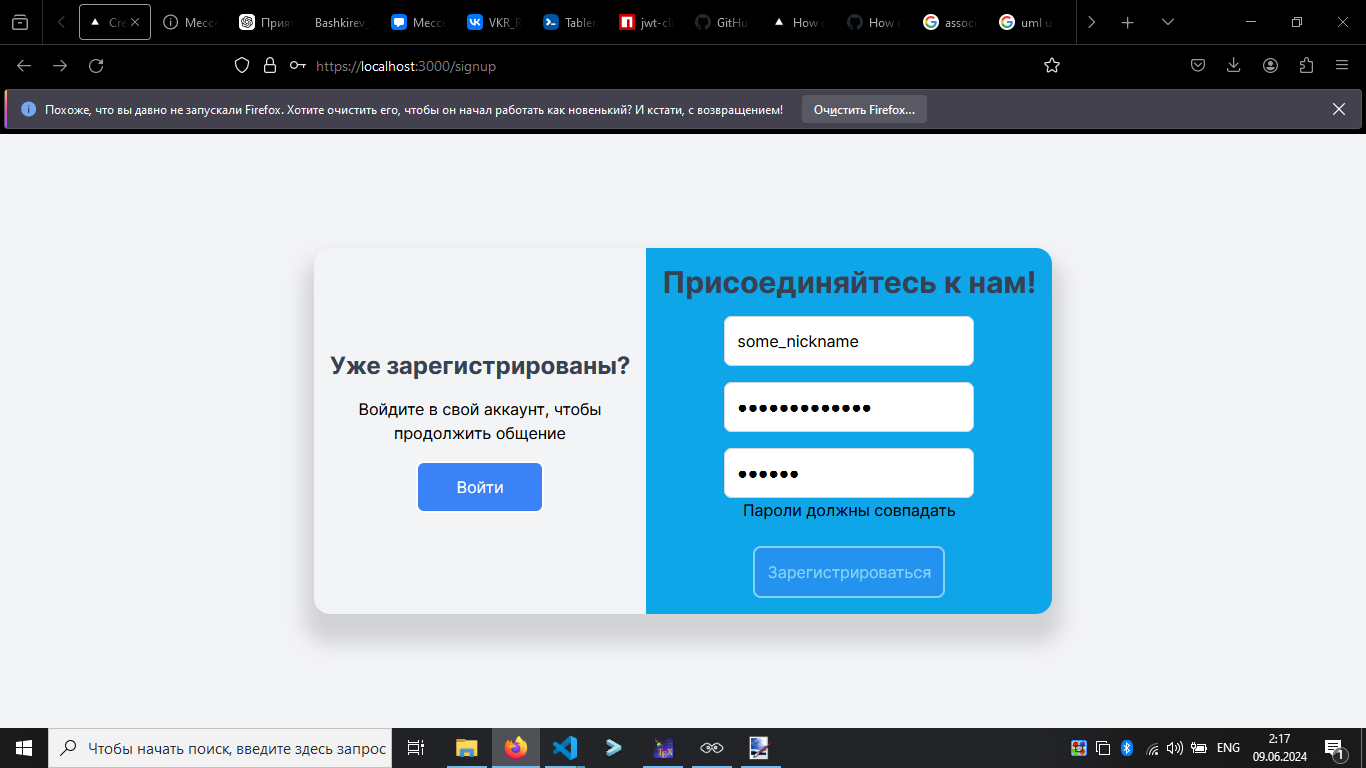
\includegraphics[width=1\linewidth]{signup_test2}}
	\caption{Попытка регистрации с неверными данными}
	\label{signup_test2:image}
\end{figure}

\begin{figure}[H]
	\center{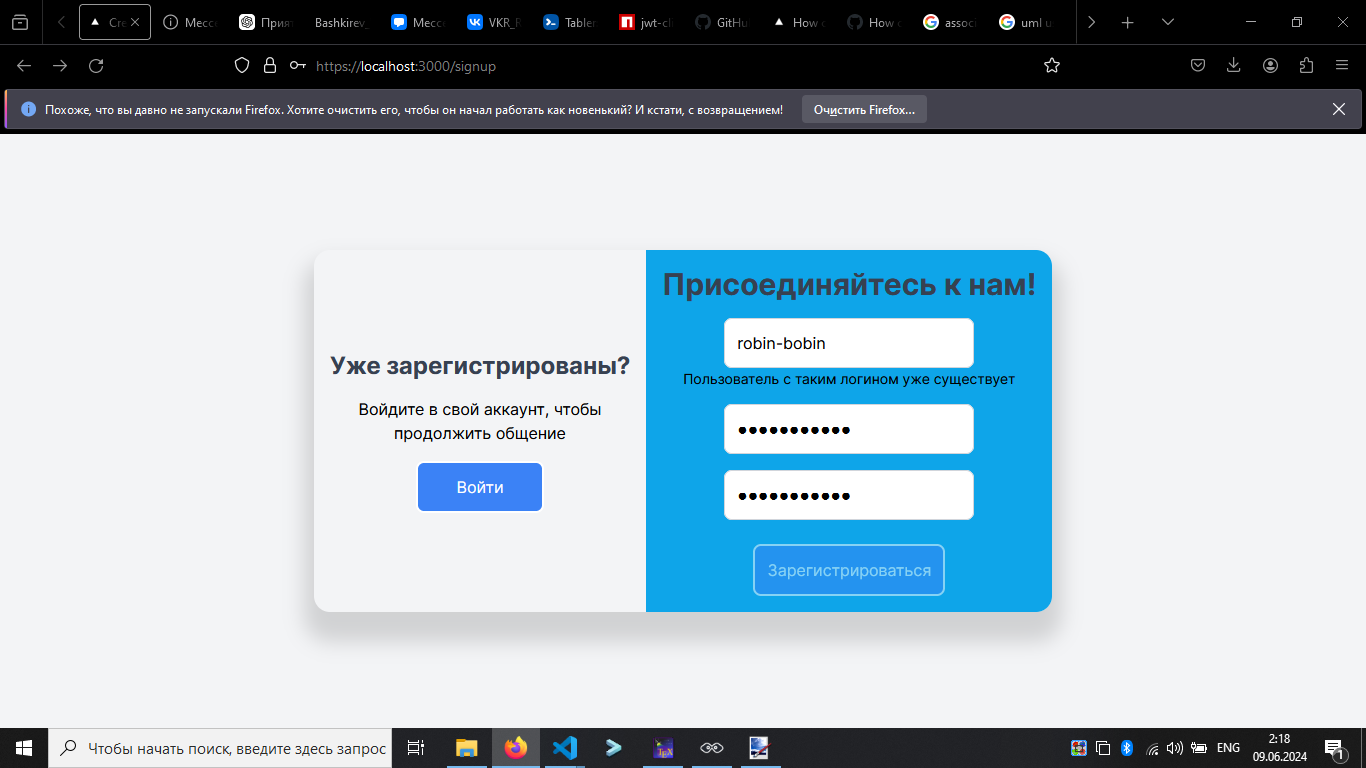
\includegraphics[width=1\linewidth]{signup_test3}}
	\caption{Попытка регистрациии с занятым логином}
	\label{signup_test3:image}
\end{figure}

После регистрации пользователь попадает на главную страницу. Результат представлен на рисунке \ref{signup_test4:image}.

\begin{figure}[H]
	\center{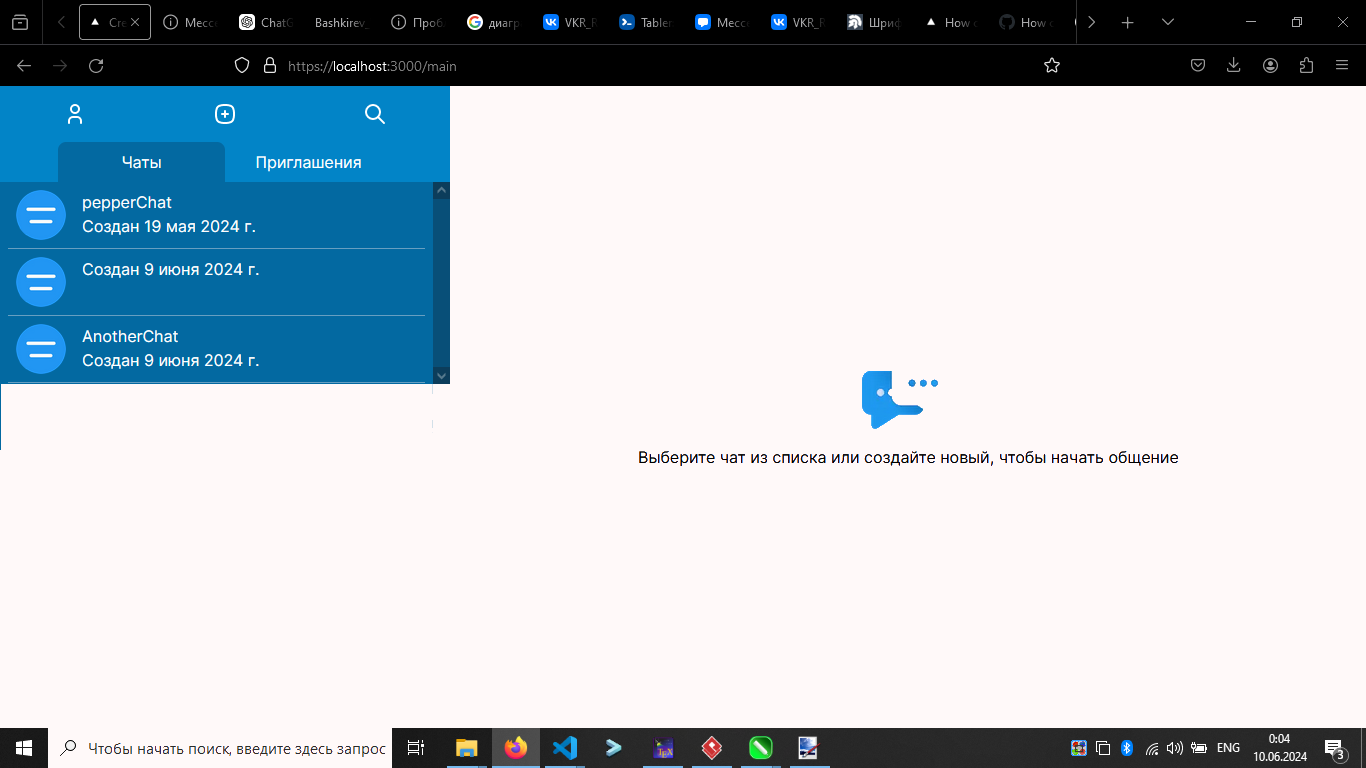
\includegraphics[width=1\linewidth]{signup_test4}}
	\caption{Переадресация на главную страницу приложения}
	\label{signup_test4:image}
\end{figure}

Приозведем тестирование функционала изменения личных данных в кабинете пользователя. Для этого попробуем изменить логин пользователя. Результаты тестирования представлены на рисунках \ref{cabinet_test1:image} и \ref{cabinet_test1:image}.


\begin{figure}[H]
	\center{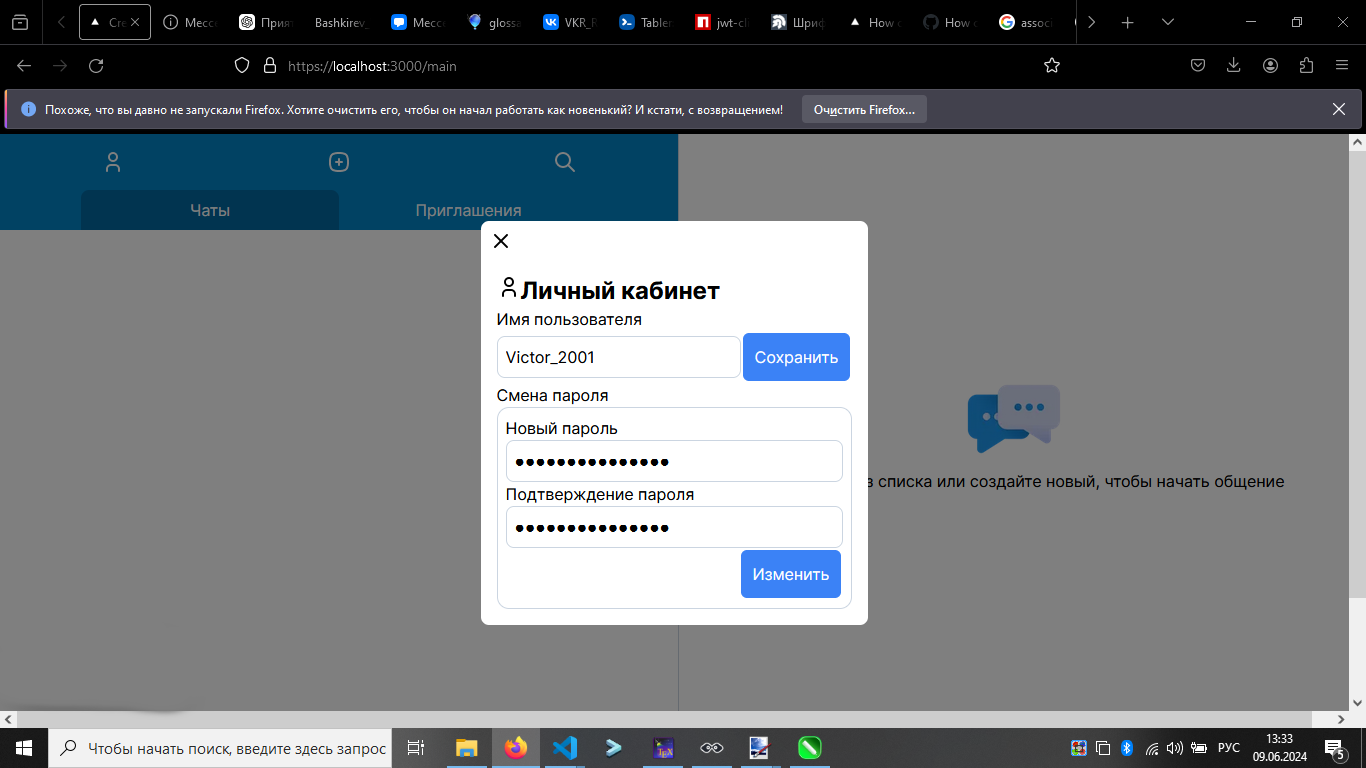
\includegraphics[width=1\linewidth]{cabinet_test1}}
	\caption{Личный кабинет пользователя с исходным логином}
	\label{cabinet_test1:image}
\end{figure}

\begin{figure}[H]
	\center{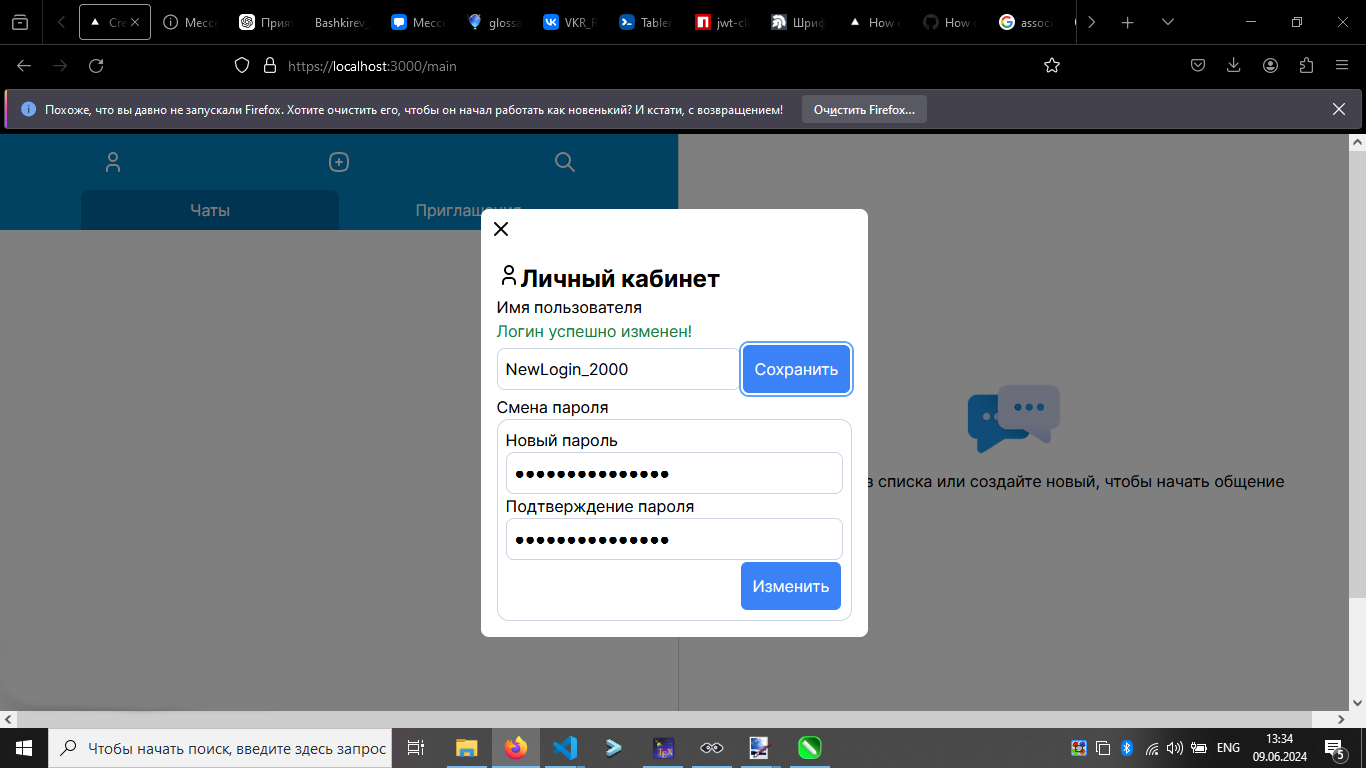
\includegraphics[width=1\linewidth]{cabinet_test2}}
	\caption{Результат изменения логина}
	\label{cabinet_test2:image}
\end{figure}

Далее протестируем функционал создания нового чата. Результаты тестов представлены на рисунках.

\begin{figure}[H]
	\center{\includegraphics[width=1\linewidth]{newChat_test1}}
	\caption{Ввод имени нового чата}
	\label{newChat_test1:image}
\end{figure}

\begin{figure}[H]
	\center{\includegraphics[width=1\linewidth]{newChat_test2}}
	\caption{Сообщение о успешном создании нового чата}
	\label{newChat_test2:image}
\end{figure}

\begin{figure}[H]
	\center{\includegraphics[width=1\linewidth]{newChat_test3}}
	\caption{Новый чат в списке чатов пользователя}
	\label{newChat_test3:image}
\end{figure}

Произведем тестирование функционала отправки сообщения. Для этого введем в поле ввода сообщения его текст и нажмем кнопку "<Отправить">. Результаты тестирования представлен на рисунках.

\begin{figure}[H]
	\center{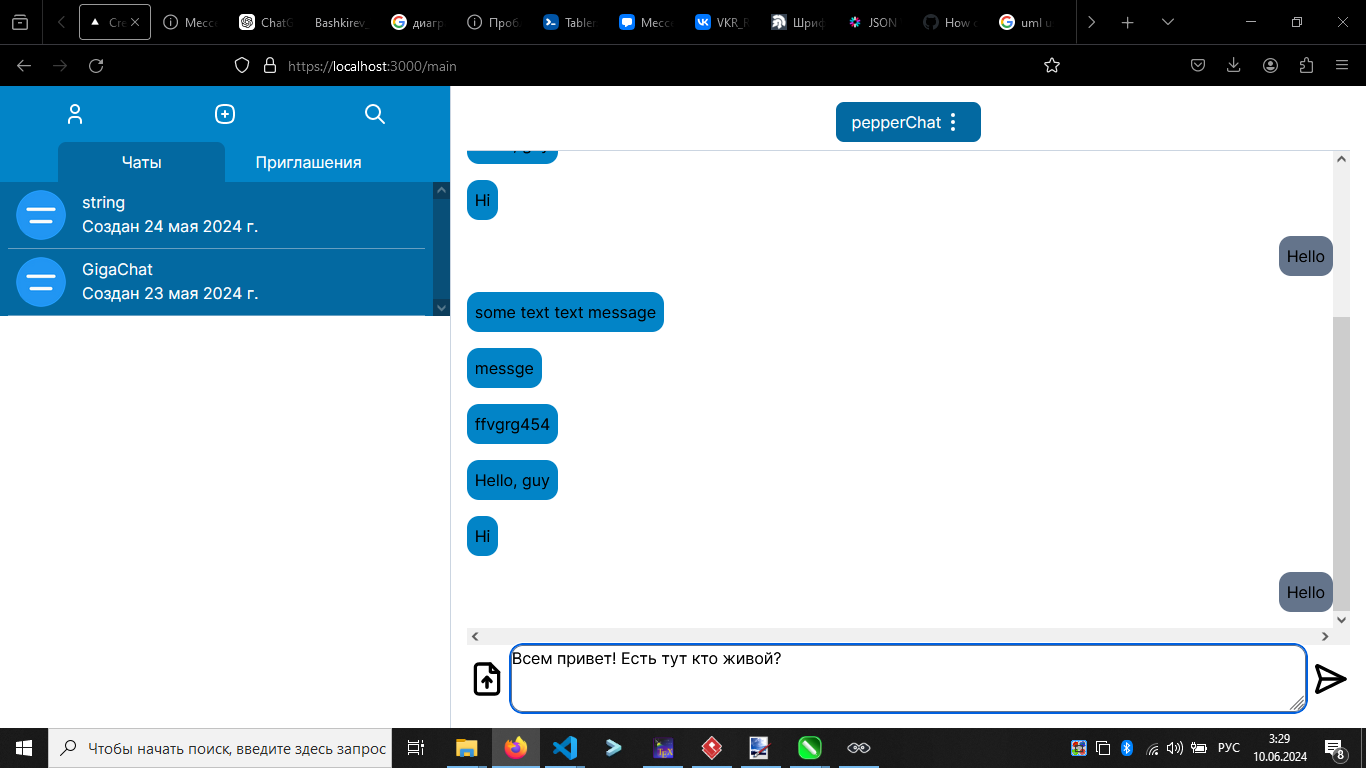
\includegraphics[width=1\linewidth]{newmessage_test1}}
	\caption{Вввод и отправка нового сообщения}
	\label{newmessage_test1:image}
\end{figure}

\begin{figure}[H]
	\center{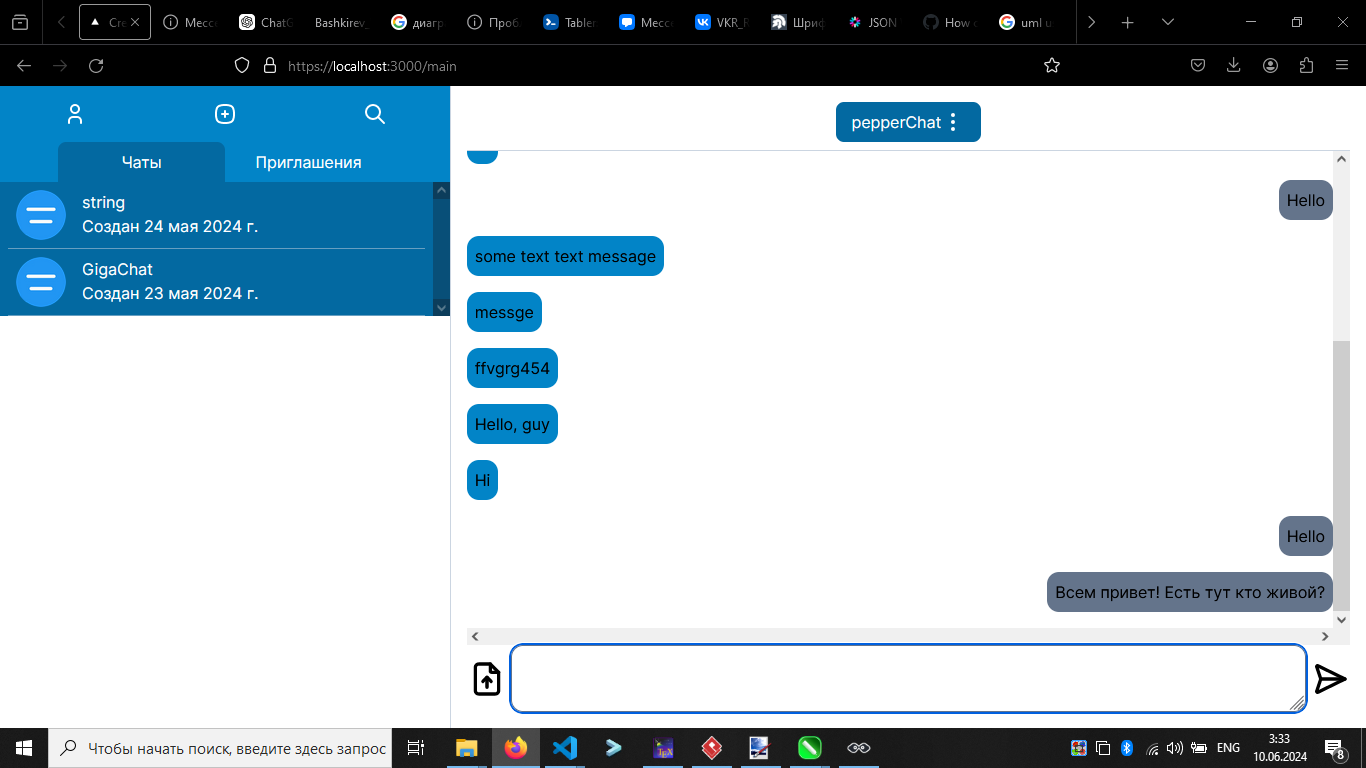
\includegraphics[width=1\linewidth]{newmessage_test2}}
	\caption{Результат отправки сообщения}
	\label{newmessage_test2:image}
\end{figure}

Произведем тестирование функционала входа в приложение. Для этого на странице входа в соответствующие поля необходимо ввести логин и пароль и нажать кнопку "<Войти">. Результаты тестирования представлены на рисунках.

\begin{figure}[H]
	\center{
\includegraphics[width=1\linewidth]{signin_test1}}
	\caption{Попытка входа с неверными данными}
	\label{signin_test1:image}
\end{figure}

\begin{figure}[H]
	\center{
\includegraphics[width=1\linewidth]{signin_test2}}
	\caption{Ввод данных пользователя}
	\label{signin_test2:image}
\end{figure}

\begin{figure}[H]
	\center{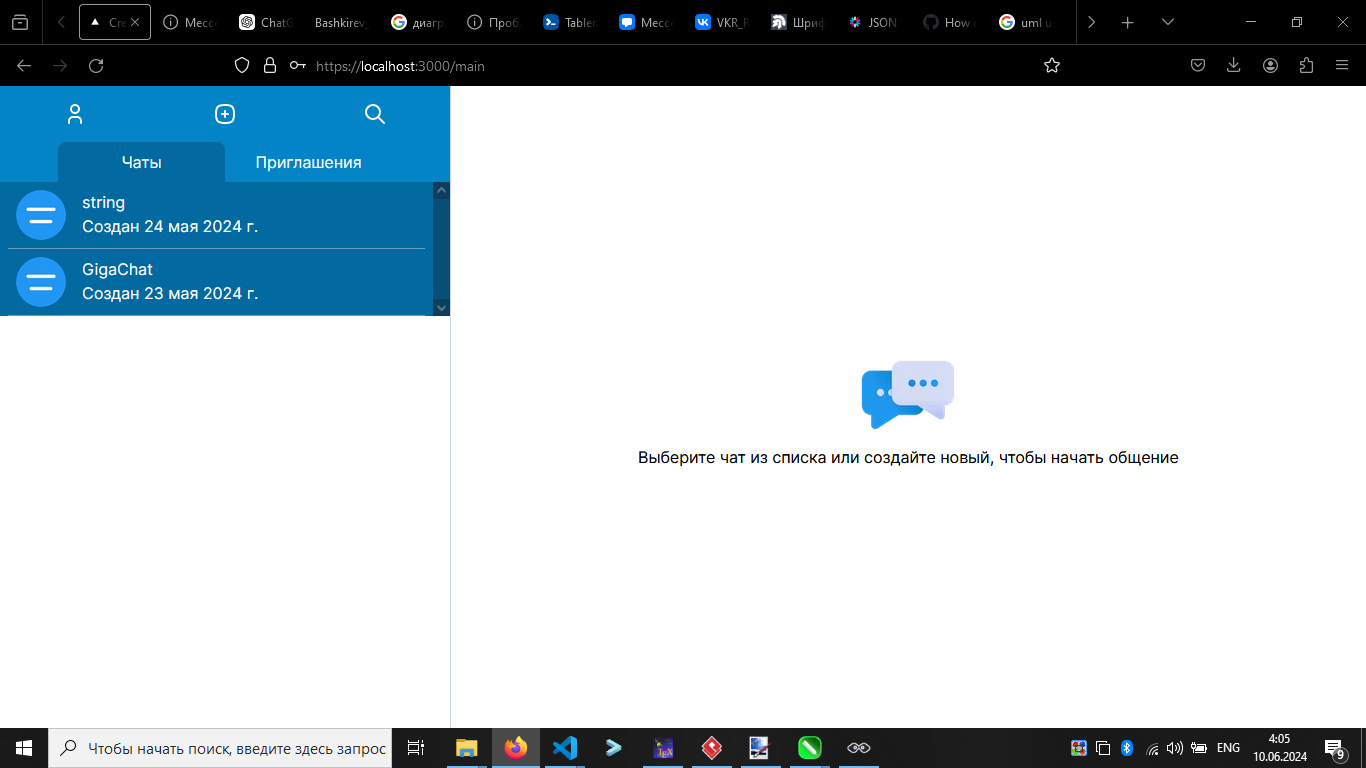
\includegraphics[width=1\linewidth]{signin_test3}}
	\caption{Главная страница после входа в приложение}
	\label{signin_test3:image}
\end{figure}
   \section*{ЗАКЛЮЧЕНИЕ}
Разработка веб-приложения чата представляет собой комплексный процесс, включающий в себя проектирование архитектуры системы, выбор технологий и инструментов, реализацию функциональных компонентов и обеспечение безопасности данных. В рамках данной дипломной работы была выполнена всесторонняя работа по созданию современного веб-приложения для обмена сообщениями.

В процессе разработки были достигнуты следующие ключевые результаты:

\begin{itemize}
	\item разработаны требования к програмнмной системе; определена модель данных и варианты импользования;
	
	\item спроектирована архитектура программной системы; определены маршруты приложения; произведен выбор технологий для программной реализации;
	
	\item реализованы модули программной системы с использованием выбранных технологий; реализован пользовательский интерфейс в виде веб-приложения для демонстрации работы приложения; проведено системное тестирование программной системы.
\end{itemize}

Итоги данной работы демонстрируют, что разработанное веб-приложение чата соответствует современным требованиям к производительности, безопасности и удобству использования. Достигнутые результаты подтверждают жизнеспособность выбранных технологий и подходов, а также их применимость для создания масштабируемых и надежных веб-приложений.

Таким образом, цели дипломной работы были успешно достигнуты, а выполненные задачи полностью соответствуют заявленной теме. Полученные результаты могут быть использованы в качестве основы для дальнейших научных исследований и практической деятельности в области веб-разработки.

}\fi
\addcontentsline{toc}{section}{СПИСОК ИСПОЛЬЗОВАННЫХ ИСТОЧНИКОВ}

\begin{thebibliography}{9}
	\bibitem{aspnetexamples} Фримен, А. ASP.NET Core 3 с примерами на C\# для профессионалов / А. Фримен. – Москва: Вильямс, 2021. – 1184 с. – 978-5-907365-46-9. – Текст~: непосредственный.
	\bibitem{cssecurity} Венц, К. Безопасность ASP. NET Core / М. Прайс. – Москва : ДМК Пресс, 2023. – 386 с. – ISBN 978-5-93700-176-4. – Текст~: непосредственный.
	\bibitem{csharp} Прайс, М. C\# 10 и .NET 6. Современная кросс-платформенная разработка / М. Прайс. – Санкт-Петербург : Питер, 2023. – 848 с. – ISBN 978-5-4461-2249-3. – Текст~: непосредственный.
	\bibitem{csdocs} Руководство по C\# | learn.microsoft.com : сайт. – URL: https://learn.microsoft.com/ru-ru/dotnet/csharp/ (дата обращения: 24.04.2024).
	\bibitem{aspnetdocs} Документация по ASP.NET | learn.microsoft.com : сайт. – URL: https://learn.microsoft.com/ru-ru/aspnet/core/?view=aspnetcore-8.0 (дата обращения: 26.04.2024).
	\bibitem{ef} Центр документации Entity Framework | learn.microsoft.com : сайт. – URL: https://learn.microsoft.com/ru-ru/ef/ (дата обращения: 25.04.2024).
	\bibitem{db} Осипов, Д.Л. Технологии проектирования баз данных / Д.Л. Осипов. – Москва : ДМК Пресс, 2019. – 498 с. – ISBN 978-5-97060-737-4. – Текст~: непосредственный.
	\bibitem{postgres} Левшин, И.В. Postgres. Первое знакомство / И.В. Левшин, П.В. Лузанов, Е.В. Рогов. – Москва : ДМК Пресс, 2023. – 178 с. – ISBN 978-5-6045970-1-9. – Текст~: непосредственный.
	\bibitem{sql} Грофф Д. Р. SQL. Полное руководство / Д. Р. Грофф, П. Н. Вайнберг, Э. Д. Опель. – 3-е изд. – Москва : Диалектика-Вильямс, 2020. – 960 с. - ISBN - 978-5-907114-26-5. Текст: непосредственный.
	\bibitem{webapi} Лоре, А. Проектирование веб-API / А. Лоре. – Москва : ДМК Пресс, 2020. – 440 с. – ISBN ISBN 978-5-97060-861-6. – Текст~: непосредственный.
	\bibitem{http} Поллард, Б. HTTP/2 в действии / Б. Поллард. – Москва~: ДМК Пресс, 2021. – 424 с. – ISBN 978-5-97060-925-5. – Текст~: непосредственный.
	\bibitem{refactor} Рефакторинг и Паттерны проектирования | refactoring.guru : сайт. – URL: https://refactoring.guru/ru (дата обращения: 08.05.2024).
	\bibitem{uml} Буч, Г. Введение в UML от создателей языка / Г. Буч, И. Якобсон, Д. Рамбо. – Москва : ДМК Пресс, 2015. – 498 с. – ISBN 978-5-457-43379-3. – Текст : непосредственный.
	\bibitem{umlproj} Флегонтов, А. В. Моделирование информационных систем. Unified Modeling Language / А.В. Флегонтов, И.Ю. Матюшичев. – Санкт-Петербург : Лань, 2023. – 140 с. – ISBN 978-5-8114-4274-4. – Текст : непосредственный.
	\bibitem{nginx} де Йонге, Д. NGINX. Книга рецептов / Д. де Йонге. – Москва~: ДМК Пресс, 2019. – 176 с. – ISBN 978-5-97060-790-9. – Текст~: непосредственный.
	\bibitem{js} Флэнаган, Д. JavaScript. Полное руководство / Д. Флэнаган. – Москва~: Диалектика-Вильямс, 2021. – 720 с. – ISBN 978-5-907203-79-2. – Текст~: непосредственный.
	\bibitem{react} Стефанов, С. React. Быстрый старт / С. Стефанов. – Санкт-Петербург : Питер, 2023. – 304 с. – ISBN 978-5-4461-2115-1. – Текст~: непосредственный.
	\bibitem{nextjs} Docs | nextjs.org : сайт. – URL: https://nextjs.org/docs (дата обращения: 06.05.2024).
	\bibitem{htmlcss} Дакетт, Дж. HTML и CSS. Разработка и дизайн веб-сайтов / Дж. Дакетт. – Москва : Эксмо, 2020 – 480 с. – ISBN 978-5-04-101286-1. – Текст~: непосредственный.
	\bibitem{webtech} Web technology for developers | developer.mozilla.org : сайт. – URL: https://developer.mozilla.org/en-US/docs/Web (дата обращения: 07.05.2024).
\end{thebibliography}
\ifВКР{\appendix{Представление графического материала}

Графический материал, выполненный на отдельных листах,
изображен на рисунках А.1--А.\arabic{числоПлакатов}.
\setcounter{числоПлакатов}{0}

\renewcommand{\thefigure}{А.\arabic{figure}} % шаблон номера для плакатов

\begin{landscape}

\begin{плакат}
    \includegraphics[width=0.82\linewidth]{sved_plakat}
    \заголовок{Сведения о ВКРБ}
    \label{sved_plakat:image}      
\end{плакат}

\begin{плакат}
    \includegraphics[width=0.82\linewidth]{tasks}
    \заголовок{Цель и задачи разработки}
    \label{tasks:image}      
\end{плакат}

\begin{плакат}
    \includegraphics[width=0.82\linewidth]{usecase_plakat}
    \заголовок{Диаграмма вариантов использования}
    \label{uscase_plakat:image}      
\end{плакат}

\begin{плакат}
    \includegraphics[width=0.82\linewidth]{comps_plakat}
    \заголовок{Диаграмма компонентов}
    \label{comps_plaket:image}      
\end{плакат}

\begin{плакат}
	\includegraphics[width=0.82\linewidth]{datamodel_plakat}
	\заголовок{Диаграмма классов модели данных}
	\label{datamodel_plakat:image}      
\end{плакат}

\begin{плакат}
	\includegraphics[width=0.82\linewidth]{controllers_plakat}
	\заголовок{Диаграмма классов контроллеров}
	\label{controllers_plakat:image}      
\end{плакат}

\begin{плакат}
	\includegraphics[width=0.82\linewidth]{routes_plakat}
	\заголовок{Карта маршрутов приложения}
	\label{routes_plakat:image}      
\end{плакат}

\begin{плакат}
	\includegraphics[width=0.82\linewidth]{zakl_plakat}
	\заголовок{Заключение}
	\label{zakl_plakat}      
\end{плакат}

\end{landscape}
}\fi
\ifПрактика{}\else{\appendix{Фрагменты исходного кода программы}

\lstdefinestyle{c#}{
	language=[Sharp]C,
	basicstyle=\ttfamily\small,
	keywordstyle=\color{blue},
	stringstyle=\color{red},
	commentstyle=\color{green},
	morecomment=[l][\color{magenta}]{\#},
	numbers=left,
	numberstyle=\tiny\color{gray},
	stepnumber=1,
	numbersep=10pt,
	backgroundcolor=\color{yellow!20},
	showspaces=false,
	showstringspaces=false,
	showtabs=false,
	frame=single,
	tabsize=4,
	captionpos=b,
	breaklines=true,
	breakatwhitespace=false,
	escapeinside={\%*}{*)},
	morekeywords={public, class, static, void, using, namespace, new, get, set, return, if, else, while, for, foreach, in, int, string, bool, true, false}
}

ChatDbContext.cs
\begin{lstlisting}[style=c#]
	using System;
	using System.Collections.Generic;
	using Microsoft.EntityFrameworkCore;
	using ChatApp.Models;
	
	namespace ChatApp;
	
	public partial class ChatDbContext : DbContext
	{
		public ChatDbContext()
		{
		}
		
		public ChatDbContext(DbContextOptions<ChatDbContext> options)
		: base(options)
		{
		}
		
		public virtual DbSet<Chat> Chats { get; set; }
		
		public virtual DbSet<Media> Media { get; set; }
		
		public virtual DbSet<Message> Messeges { get; set; }
		
		public virtual DbSet<User> Users { get; set; }
		
		public virtual DbSet<UserRole> UserRoles { get; set; }
		
		public virtual DbSet<UsersInChats> UsersInChats { get; set; }
		
		protected override void OnConfiguring(DbContextOptionsBuilder optionsBuilder)
		=> optionsBuilder.UseNpgsql("Name=ConnectionStrings:DBConnection");
		
		protected override void OnModelCreating(ModelBuilder modelBuilder)
		{
			modelBuilder.Entity<Chat>(entity =>
			{
				entity.HasKey(e => e.ChatId).HasName("chats_pkey");
				
				entity.ToTable("chats");
				
				entity.Property(e => e.ChatId).HasColumnName("chat_id");
				entity.Property(e => e.CreationDate).HasColumnName("creation_date");
				entity.Property(e => e.Name)
				.HasMaxLength(128)
				.HasColumnName("name");
			});
			
			modelBuilder.Entity<Media>(entity =>
			{
				entity.HasKey(e => e.MediaId).HasName("media_pkey");
				
				entity.ToTable("media");
				
				entity.Property(e => e.MediaId).HasColumnName("media_id");
				entity.Property(e => e.Location).HasColumnName("location");
				entity.Property(e => e.MessegeId).HasColumnName("messege_id");
				
				entity.HasOne(d => d.Messege).WithMany(p => p.Media)
				.HasForeignKey(d => d.MessegeId)
				.OnDelete(DeleteBehavior.ClientSetNull)
				.HasConstraintName("messege_id");
			});
			
			modelBuilder.Entity<Message>(entity =>
			{
				entity.HasKey(e => e.MessageId).HasName("messeges_pkey");
				
				entity.ToTable("messeges");
				
				entity.Property(e => e.MessageId).HasColumnName("messege_id");
				entity.Property(e => e.ChatId).HasColumnName("chat_id");
				entity.Property(e => e.Content).HasColumnName("content");
				entity.Property(e => e.UserId).HasColumnName("user_id");
				
				entity.HasOne(d => d.Chat).WithMany(p => p.Messeges)
				.HasForeignKey(d => d.ChatId)
				.OnDelete(DeleteBehavior.ClientSetNull)
				.HasConstraintName("chat_fkey");
				
				entity.HasOne(d => d.User).WithMany(p => p.Messeges)
				.HasForeignKey(d => d.UserId)
				.OnDelete(DeleteBehavior.SetNull)
				.HasConstraintName("user_fkey");
			});
			
			modelBuilder.Entity<User>(entity =>
			{
				entity.HasKey(e => e.UserId).HasName("users_pkey");
				
				entity.ToTable("users");
				
				entity.Property(e => e.UserId).HasColumnName("user_id");
				entity.Property(e => e.Login)
				.HasMaxLength(64)
				.HasColumnName("login");
				entity.Property(e => e.PasswordHash).HasColumnName("password_hash");
				entity.Property(e => e.PasswordSalt).HasColumnName("password_salt");
			});
			
			modelBuilder.Entity<UserRole>(entity =>
			{
				entity.HasKey(e => e.RoleId).HasName("user_role_pkey");
				
				entity.ToTable("user_role");
				
				entity.Property(e => e.RoleId)
				.ValueGeneratedNever()
				.HasColumnName("role_id");
				entity.Property(e => e.RoleName)
				.HasMaxLength(15)
				.HasColumnName("role_name");
			});
			
			modelBuilder.Entity<UsersInChats>(entity =>
			{
				entity.HasKey(e => new { e.UserId, e.ChatId }).HasName("users_in_chats_pkey");
				
				entity.ToTable("users_in_chats");
				
				entity.Property(e => e.UserId).HasColumnName("user_id");
				entity.Property(e => e.ChatId).HasColumnName("chat_id");
				entity.Property(e => e.UserRole).HasColumnName("user_role");
				
				entity.HasOne(d => d.Chat).WithMany(p => p.UsersInChats)
				.HasForeignKey(d => d.ChatId)
				.HasConstraintName("chat_fkey");
				
				entity.HasOne(d => d.User).WithMany(p => p.UsersInChats)
				.HasForeignKey(d => d.UserId)
				.HasConstraintName("user_fkey");
				
				entity.HasOne(d => d.UserRoleNavigation).WithMany(p => p.UsersInChats)
				.HasForeignKey(d => d.UserRole)
				.OnDelete(DeleteBehavior.ClientSetNull)
				.HasConstraintName("user_role_fkey");
			});
			
			OnModelCreatingPartial(modelBuilder);
		}
		
		partial void OnModelCreatingPartial(ModelBuilder modelBuilder);
	}	
\end{lstlisting}

AuthController.cs
\begin{lstlisting}[style=c#]
	using System.Security.Cryptography;
	using System.Text;
	using AuthService.Models;
	using AuthService.Models.DTOs;
	using AuthService.Models.Requsets;
	using AuthService.Services;
	using AutoMapper;
	using Microsoft.AspNetCore.Mvc;
	using Microsoft.EntityFrameworkCore;
	using RandomString4Net;
	
	namespace AuthService.Controllers;
	
	[Route("api/[controller]")]
	[ApiController]
	public class AuthController : ControllerBase
	{
		private readonly ChatDbContext dbContext;
		private readonly JwtService jwtService;
		private readonly IMapper mapper;
		public AuthController(ChatDbContext dbContext, JwtService jwtService, IMapper mapper)
		{
			this.dbContext = dbContext;
			this.jwtService = jwtService;
			this.mapper = mapper;
		}
		
		[HttpPost("signup")]
		public async Task<IActionResult> SignUp(AccountRequest regData)
		{
			if (dbContext.Users.SingleOrDefault(u => u.Login == regData.Login) != null)
			{
				return Conflict("User already exist");
			}
			string salt = RandomString.GetString(Types.ALPHANUMERIC_MIXEDCASE, 10);
			
			byte[] passwordHash = SHA256.HashData(Encoding.UTF8.GetBytes(regData.Password + salt));
			
			User newUser = new User
			{
				Login = regData.Login,
				PasswordHash = passwordHash,
				PasswordSalt = Encoding.UTF8.GetBytes(salt)
			};
			
			await dbContext.Users.AddAsync(newUser);
			try
			{
				await dbContext.SaveChangesAsync();
			}
			catch(Exception e)
			{
				Console.WriteLine(e);
				return StatusCode(500);
			}
			
			string refreshToken = jwtService.GetRefreshToken(newUser.UserId);
			string accessToken = jwtService.GetAccessToken(newUser.UserId, newUser.Login);
			
			HttpContext.Response.Headers.Authorization = "Bearer " + accessToken;
			
			return Ok("Bearer " + refreshToken);
		}
		
		[HttpPost("signin")]
		public async Task<IActionResult> SignIn([FromBody]AccountRequest account)
		{
			User? user = await dbContext.Users
			.SingleOrDefaultAsync(u => u.Login == account.Login);
			
			if (user == null)
			{
				return NotFound();
			}
			
			string salt = Encoding.UTF8.GetString(user.PasswordSalt);
			
			byte[] hash = SHA256.HashData(Encoding.UTF8.GetBytes(account.Password + salt));
			
			if (!hash.SequenceEqual(user.PasswordHash))
			{
				return Unauthorized();
			}
			
			string refreshToken = jwtService.GetRefreshToken(user.UserId);
			string accessToken = jwtService.GetAccessToken(user.UserId, user.Login);
			
			HttpContext.Response.Headers.Authorization = "Bearer " + accessToken;
			
			return Ok("Bearer " + refreshToken);
		}
	}
\end{lstlisting}

TokensController.cs
\begin{lstlisting}[style=c#]
	using System.Security.Claims;
	using AuthService.Models;
	using AuthService.Models.Requsets;
	using AuthService.Services;
	using Microsoft.AspNetCore.Authorization;
	using Microsoft.AspNetCore.Mvc;
	
	[Route("api/[controller]")]
	[ApiController]
	[Authorize(AuthenticationSchemes = "RefreshTokenScheme")]
	public class TokensController : ControllerBase
	{
		private readonly ChatDbContext dbContext;
		private readonly JwtService jwtService;
		public TokensController(ChatDbContext dbContext, JwtService jwtService)
		{
			this.dbContext = dbContext;
			this.jwtService = jwtService;
		}
		
		[HttpGet("chat-token/{id:int}")]
		public async Task<IActionResult> GetChatToken(int id)
		{
			int userId = Int32.Parse(HttpContext.User.FindFirst(ClaimTypes.NameIdentifier)?.Value!);
			var user = await dbContext.Users.FindAsync(userId);
			
			var userChat = user.UsersInChats.SingleOrDefault(x => x.ChatId == id);
			
			if (userChat == null)
			{
				return Unauthorized();
			}
			
			var role = userChat
			.UserRoleNavigation;
			
			string chatToken = jwtService.GetChatToken(userChat.UserId, userChat.ChatId, role);
			
			HttpContext.Response.Headers.Authorization = chatToken;
			
			return Ok(new { ChatId = id, UserId = user.UserId, Role = role.RoleName });
		}
		
		[HttpGet("refresh-access-token")]
		public async Task<IActionResult> RefreshAccessToken()
		{
			int id = Int32.Parse(HttpContext.User.FindFirst(ClaimTypes.NameIdentifier)?.Value!);
			var user = await dbContext.Users.FindAsync(id);
			string token = "Bearer " + jwtService.GetAccessToken(user.UserId, user.Login);
			
			HttpContext.Response.Headers.Authorization = token;
			
			return NoContent();
		}
		
		[HttpGet("refresh-chat-token")]
		public async Task<IActionResult> RefreshChatToken(string chatToken)
		{
			
			var claimsPrincipal = (ClaimsPrincipal)HttpContext.Items["ClaimsPrincipal"]!;
			
			int id = Int32.Parse(claimsPrincipal.FindFirst(ClaimTypes.NameIdentifier)?.Value!);
			var user = await dbContext.Users.FindAsync(id);
			
			int chatId = Int32.Parse(claimsPrincipal.FindFirst("chatId")?.Value!);
			
			var userChatInfo = user?.UsersInChats.Single(item => item.ChatId == chatId);
			
			string newToken = jwtService.GetChatToken(id, userChatInfo.ChatId, userChatInfo.UserRoleNavigation);
			
			return Ok(newToken);
		}
	}
\end{lstlisting}

JwtService.cs
\begin{lstlisting}[style=c#]
	using System.IdentityModel.Tokens.Jwt;
	using System.Security.Claims;
	using System.Text;
	using AuthService.Models;
	using AuthService.Models.Requsets;
	using Microsoft.IdentityModel.Tokens;
	
	namespace AuthService.Services;
	
	public class JwtService
	{
		private readonly IConfiguration configuration;
		
		public JwtService(IConfiguration config)
		{
			configuration = config;
		}
		
		public string GetAccessToken(int id, string login)
		{
			var tokenHandler = new JwtSecurityTokenHandler();
			byte[] secret = Encoding.UTF8.GetBytes(configuration["JwtSettings:AppKey"]!);
			
			var tokenDescriptor = new SecurityTokenDescriptor
			{
				Subject = new ClaimsIdentity(new Claim[]
				{
					new Claim(ClaimTypes.NameIdentifier, id.ToString()),
					new Claim(ClaimTypes.Name, login)
				}),
				IssuedAt = DateTime.Now,
				Issuer = configuration["JwtSettings:Issuer"],
				Expires = DateTime.Now.AddMinutes(30),
				SigningCredentials = new SigningCredentials(new SymmetricSecurityKey(secret), SecurityAlgorithms.HmacSha256)
			};
			
			var token = tokenHandler.CreateToken(tokenDescriptor);
			
			return tokenHandler.WriteToken(token);
		}
		
		public string GetRefreshToken(int id)
		{
			var tokenHandler = new JwtSecurityTokenHandler();
			byte[] secret = Encoding.UTF8.GetBytes(configuration["JwtSettings:AppKey"]!);
			
			var tokenDescriptor = new SecurityTokenDescriptor
			{
				Subject = new ClaimsIdentity(
				[
				new Claim(ClaimTypes.NameIdentifier, id.ToString()),
				]),
				Issuer = configuration["JwtSettings:Issuer"],
				IssuedAt = DateTime.Now,
				Expires = DateTime.Now.AddDays(1),
				SigningCredentials = new SigningCredentials(new SymmetricSecurityKey(secret), SecurityAlgorithms.HmacSha256)
			};
			
			var token = tokenHandler.CreateToken(tokenDescriptor);
			
			return tokenHandler.WriteToken(token);
		}
		
		public string GetChatToken(int userId, int chatId, UserRole userRole)
		{
			byte[] secret = Encoding.UTF8.GetBytes(configuration["JwtSettings:ChatsKey"]!);
			
			var claims = new List<Claim>
			{
				new Claim(type: ClaimTypes.NameIdentifier, value: userId.ToString()),
				new Claim(type: "chatId", value: chatId.ToString()),
				new Claim(type: ClaimTypes.Role, value: userRole.RoleName)
			};
			
			var key = new SymmetricSecurityKey(secret);
			var creds = new SigningCredentials(key, SecurityAlgorithms.HmacSha256);
			
			var token = new JwtSecurityToken(
			issuer: configuration["JwtSettings:Issuer"],
			claims: claims,
			expires: DateTime.Now.AddMinutes(30),
			signingCredentials: creds);
			
			return new JwtSecurityTokenHandler().WriteToken(token);
		}
	}
\end{lstlisting}

ChatController.cs
\begin{lstlisting}[style=c#]
	using System.Security.Claims;
	using AutoMapper;
	using ChatApp;
	using ChatApp.Models;
	using ChatApp.Models.Requests;
	using Microsoft.AspNetCore.Authorization;
	using Microsoft.AspNetCore.Mvc;
	using Microsoft.AspNetCore.SignalR;
	
	
	[Route("api/[controller]")]
	[ApiController]
	[Authorize]
	[GetIdentifiersFilter]
	public class ChatController : Controller
	{
		private readonly ChatDbContext dbContext;
		private readonly IHubContext<ChatHub> hubContext;
		private readonly IMapper mapper;
		
		public ChatController(ChatDbContext dbContext, IHubContext<ChatHub> hubContext, IMapper mapper)
		{
			this.dbContext = dbContext;
			this.hubContext = hubContext;
			this.mapper = mapper;
		}
		
		[HttpPost("send-message")]
		public async Task<IActionResult> SendMessage([FromBody] SendMessageRequest newMessage)
		{
			int userId = (int)HttpContext.Items["UserId"]!;
			int chatId = (int)HttpContext.Items["ChatId"]!;
			
			Chat chat = await dbContext.Chats.FindAsync(chatId);
			User user = await dbContext.Users.FindAsync(userId);
			
			Message message = new Message
			{
				ChatId = chatId,
				UserId = userId,
				Content = newMessage.Content,
				Chat = chat,
				User = user
			};
			
			await dbContext.Messeges.AddAsync(message);
			chat.Messeges.Add(message);
			
			await dbContext.SaveChangesAsync();
			
			await hubContext.Clients
			.Group(chat.Name)
			.SendAsync("NewMessage", newMessage.Content);
			
			return Ok();
		}
		
		[HttpDelete("delete-message")]
		public async Task<IActionResult> DeleteMessage([FromBody] DeleteMessageRequest toDelete)
		{
			int chatId = (int)HttpContext.Items["ChatId"]!;
			
			Chat chat = await dbContext.Chats.FindAsync(chatId);
			Message message = await dbContext.Messeges.FindAsync(toDelete.MessageId);
			
			chat.Messeges.Remove(message);
			dbContext.Messeges.Remove(message);
			
			await dbContext.SaveChangesAsync();
			
			await hubContext.Clients
			.Group(chat.Name)
			.SendAsync("NewMessage", toDelete.MessageId);
			
			return Ok();
		}
		
		[HttpGet("messages")]
		public async Task<IActionResult> GetMesseges()
		{
			int chatId = (int)HttpContext.Items["ChatId"]!;
			
			Chat? chat = await dbContext.Chats.FindAsync(chatId);
			
			return Ok(chat.Messeges);
		}
		
		[HttpGet("users")]
		public async Task<IActionResult> GetUsers()
		{
			int chatId = (int)HttpContext.Items["ChatId"]!;
			
			Chat? chat = await dbContext.Chats.FindAsync(chatId);
			
			var users = chat.UsersInChats
			.Select((item) => item.User)
			.ToList();
			
			return Ok(users);        
		}
		
		[HttpDelete("delete-user")]
		public async Task<IActionResult> DeleteUser([FromBody] DeleteUserRequest toDelete)
		{
			int chatId = (int)HttpContext.Items["ChatId"]!;
			
			Chat? chat = await dbContext.Chats.FindAsync(chatId);
			UsersInChats userInChat = chat.UsersInChats.Single((item) => item.UserId == toDelete.UserId);
			
			chat.UsersInChats.Remove(userInChat);
			dbContext.UsersInChats.Remove(userInChat);
			
			await dbContext.SaveChangesAsync();
			
			await hubContext.Clients
			.Group(chat.Name)
			.SendAsync("UserDeleted", userInChat.User.Login);
			
			return Ok();
		}
	}
\end{lstlisting}

ChatsController.cs
\begin{lstlisting}[style=c#]
	using System.Security.Claims;
	using AutoMapper;
	using ChatApp.Models;
	using ChatApp.Models.Requests;
	using ChatApp.Models.DTOs;
	using Microsoft.AspNetCore.Authorization;
	using Microsoft.AspNetCore.Mvc;
	
	namespace ChatApp.Controllers
	{
		
		[Route("/api/[controller]")]
		[ApiController]
		public class ChatsController : ControllerBase
		{
			private readonly ChatDbContext dbContext;
			private readonly IMapper mapper;
			public ChatsController(ChatDbContext dbContext, IMapper mapper)
			{
				this.dbContext = dbContext;
				this.mapper = mapper;
			}
			
			[Authorize]
			[HttpPost]
			public async Task<IActionResult> AddNewChat([FromBody] NewChatRequest request)
			{
				Chat newChat = new Chat
				{
					Name = request.ChatName,
					CreationDate = DateOnly.FromDateTime(DateTime.Now)
				};
				
				await dbContext.Chats.AddAsync(newChat);
				await dbContext.SaveChangesAsync();
				
				int userId = Int32.Parse(HttpContext.User.FindFirst(ClaimTypes.NameIdentifier)?.Value!);
				var user = await dbContext.Users.FindAsync(userId)!;
				
				await dbContext.UsersInChats.AddAsync(new UsersInChats
				{
					User = user,
					UserId = user.UserId,
					Chat = newChat,
					ChatId = newChat.ChatId,
					UserRole = (int)UserRolesEnum.Admin
				});
				
				await dbContext.SaveChangesAsync();
				
				return Ok(mapper.Map<ChatInfoDto>(newChat));
			}
			
			[Authorize(Roles = "admin", Policy = "ChatsTokenPolicy")]
			[HttpDelete]
			public async Task<IActionResult> DeleteChat([FromBody] DeleteChatRequest toDelete)
			{
				Chat? chat = await dbContext.Chats.FindAsync(toDelete.ChatId);
				
				if (chat == null)
				{
					return NotFound();
				}
				
				dbContext.Chats.Remove(chat);
				
				await dbContext.SaveChangesAsync();
				
				return Ok();
			}
			
			
			[Authorize]
			[HttpGet("{id:int}")]
			public async Task<IActionResult> GetChatInfo(int id)
			{
				var chat = await dbContext.Chats.FindAsync(id);
				
				if (chat == null)
				{
					return NotFound();
				}
				
				
				return Ok(mapper.Map<ChatInfoDto>(chat));
			}
		}
		
	}
\end{lstlisting}

SignUpPage.tsx
\begin{lstlisting}[language=javascript]
	'use client'
	
	import { UserInfo } from "@/models/userInfo";
	import axios from "axios";
	import { ErrorMessage, Field, Form, Formik, FormikHelpers } from "formik";
	import { useRouter } from "next/navigation";
	import { ReactNode } from "react";
	import * as Yup from 'yup';
	
	const authUrl = process.env.NEXT_PUBLIC_AUTH_URL;
	
	type SignUpValues= {
		login: string, 
		password: string,
		confirmPassword: string,
		general?: string
	};
	
	const schema = Yup.object().shape({
		login: Yup.string()
		.min(8, "Имя пользователя должно содержать не менее 8 символов")
		.max(32, "Имя пользователя должно содержать не более 32 символов")
		.required("Введите имя пользователя"),
		password: Yup.string()
		.min(8, "Пароль должен содержать не менее 8 символов")
		.max(64, "Пароль должен содержать не более 64 символов")
		.required("Введите пароль"),
		confirmPassword: Yup.string()
		.oneOf([Yup.ref('password')], "Пароли должны совпадать")
		.required("Подтвердите свой пароль")
	});
	
	export default function SignUpPage(){
		const router = useRouter();
		
		const initialValues = {
			login: "",
			password: "",
			confirmPassword: ""
		};
		
		const handleOnSubmit = async ({ login, password }:SignUpValues,
		{ setSubmitting, setErrors }: FormikHelpers<SignUpValues>
		) => {
			try{
				const {headers} = await axios.post<UserInfo>(`${authUrl}/Auth/signup`, {login, password})
				
				localStorage.setItem("Access-Token", headers["authorization"]);
				
				router.push("/main");
			}
			catch(error){
				if (axios.isAxiosError(error)){
					if (error.response?.status == 409){
						setErrors({login: "Пользователь с таким логином уже существует"})
					}
					if(error.response?.status == 500){
						setErrors({general: "Произошла неизвестная ошибка. Попробуйте еще раз"})
					}
				}
			}
			finally{
				setSubmitting(false);
			}
		}
		
		return (
		<div className="flex flex-grow-0 flex-col-reverse md:flex-row justify-between items-center md:rounded-2xl md:max-w-min md:min-h-max shadow-[0px_20px_20px_10px_#00000024] overflow-hidden">
		<div className="flex flex-col items-center justify-center text-center self-stretch m-4">
		<h3 className="text-2xl font-bold md:text-nowrap text-gray-700 mb-4 block">Уже зарегистрированы?</h3>
		<p className="block mb-4">Войдите в свой аккаунт, чтобы продолжить общение</p>
		<a href="/signin" className="w-full p-3 bg-blue-500 text-white rounded-lg border-2 border-white max-w-32 hover:bg-blue-600 focus:outline-none focus:ring-2 focus:ring-blue-400">
		Войти
		</a>
		</div>
		<div className="flex flex-grow-0 justify-center bg-sky-500">
		<div className="flex flex-col items-center text-center m-4 min-h-full">
		<h3 className="text-3xl md:text-nowrap font-bold text-gray-700 mb-4" >Присоединяйтесь к нам!</h3>
		<Formik initialValues={initialValues}
		validationSchema={schema}
		onSubmit={handleOnSubmit}
		>
		{({isSubmitting, errors, isValid}) => (
			<Form className="flex flex-col items-center min-h-max">
			<div className="mb-4">
			<Field
			type="text"
			name="login"
			placeholder="Имя пользователя"
			className="p-3 border md:w-[250px] border-gray-300 rounded-lg focus:outline-none focus:ring-2 focus:ring-blue-400"
			/>
			<ErrorMessage component={ErrorTemplate} name="login" />
			</div>
			<div className="mb-4">
			<Field
			type="password"
			name="password"
			placeholder="Пароль"
			className="md:w-[250px] p-3 border border-gray-300 rounded-lg focus:outline-none focus:ring-2 focus:ring-blue-400"
			/>
			<ErrorMessage component={ErrorTemplate} name="password" />
			</div>
			<div className="mb-6">
			<Field
			type="password"
			name="confirmPassword"
			placeholder="Повторите пароль"
			className="md:w-[250px] p-3 border border-gray-300 rounded-lg focus:outline-none focus:ring-2 focus:ring-blue-400"
			/>
			<div>
			<ErrorMessage name="confirmPassword" />
			</div>
			</div>
			<button
			type="submit"
			disabled={isSubmitting || !isValid}
			className="w-fit py-3 px-3 bg-blue-500 text-white rounded-lg border-2 border-white disabled:opacity-50 disabled:cursor-not-allowed disabled:pointer-events-none hover:bg-blue-600 focus:outline-none focus:ring-2 focus:ring-blue-400"
			>
			{isSubmitting == true ? "Регистрируем вас..." : "Зарегистрироваться"}
			</button>
			<div>
			{errors.general && <p className="text-center text-wrap">{errors.general}</p>}
			</div>
			</Form>
			)}
		</Formik>
		</div>
		</div>
		</div>
		);
	};
	
	function ErrorTemplate({children}:{children?: ReactNode}){
		return(
		<div className="text-center break-words max-w-full text-sm">
		<p>{children}</p>
		</div>
		)
	}
\end{lstlisting}

ChatRoom.tsx
\begin{lstlisting}[language=javascript]
	import { useSelectedChatContext } from "@/context/selectedChatContext";
	import Image from "next/image";
	import noChatPlaceholder from "../../public/img/no-chat.png";
	import { IconDotsVertical, IconFileUpload, IconSend2 } from "@tabler/icons-react";
	import { useEffect, useRef, useState } from "react";
	import axios, { AxiosRequestConfig } from "axios";
	import { Chat } from "@/models/chat";
	import Messages from "./Messages";
	import { Spinner } from "./Spinner";
	import { Modal } from "./Modal";
	import { HubConnectionBuilder } from "@microsoft/signalr";
	import { useChatContext, useChatContextProvider } from "@/context/chatContext";
	import { decodeToken } from "@/utils/decodeToken";
	import { ChatUser } from "@/models/chatUser";
	import { useHubConnectionContext } from "@/context/hubConnectionContext";
	import { Field, Form, Formik, FormikHelpers, FormikValues } from "formik";
	import jwtClient from "jwt-client"; 
	import { jwtDecode } from "jwt-decode";
	
	const apiUrl = process.env.NEXT_PUBLIC_API_URL;
	const authUrl = process.env.NEXT_PUBLIC_AUTH_URL;
	
	type ChatProps = {
		title: string
	};
	
	type MessageFormValues = {
		message: string
	};
	
	export default function ChatRoom(){
		const {chatId} = useSelectedChatContext();
		const [chat, setChat] = useState<ChatUser>();
		const [chatInfo, setChatInfo] = useState<Chat>();
		const ChatProvider = useChatContextProvider();
		
		useEffect(() =>{
			axios.get<Chat>(`${apiUrl}/Chats/${chatId}`, {
				headers: {
					"Authorization" : localStorage.getItem(`Access-Token`)
				}, 
				withCredentials: true
			}).then((res) => {
				setChatInfo(res.data)
			})
		}, [chat]);
		
		useEffect(() =>{
			if (!chatId){
				return;
			}
			
			axios.get<ChatUser>(`${authUrl}/Tokens/chat-token/${chatId}`, {
				withCredentials: true,
				headers: {
					"Authorization": localStorage.getItem("Refresh-Token")
				}
			})
			.then((res) => {
				const chatToken: string = res.headers["authorization"];
				localStorage.setItem(`Chat-Token-${chatId}`, chatToken);
				
				setChat(res.data);
				
			}).catch((reason) => console.log(reason));
			
		}, [chatId]);
		
		if (!chatId){
			return <NoChat/>
		}
		
		if (!chatInfo){
			return <Spinner text="Загружаем данные чата..."/>
		}
		
		if (chatInfo){
			return (
			<ChatProvider value={chat!}>
			<Chat title={chatInfo.title}/>
			</ChatProvider>
			)
		}
	}
	
	function Chat({title}:ChatProps){
		const [active, setActive] = useState(false);
		const chatId = useSelectedChatContext();
		
		const initValues = {
			message: ""
		}
		
		const handleOnSubmit = async ({message}:MessageFormValues) => {
			await axios.post(`${apiUrl}/Chat/send-message`, {
				content: message
			}, {
				withCredentials: true,
				headers: {
					"Authorization": localStorage.getItem("Access-Token")
				}
			})
		}
		
		return(
		<div className="flex flex-col w-full h-full">
		<div className="flex flex-col p-4 justify-center items-center w-full h-full">
		<div className="flex items-center justify-center w-full border-slate-300 border-b border-solid pb-2">
		<div className="flex text-center bg-sky-700 py-2 px-4 text-white rounded-lg">
		<p>{title}</p>
		<button onClick={() => setActive(true)}><IconDotsVertical/></button>
		</div>
		</div>
		<Messages/>
		<div className="flex gap-1 justify-between max-h-min w-full items-center"> {/* Добавлено items-center */}
		<button className="flex items-center w-max h-full"><IconFileUpload className="h-10 w-10" /></button> {/* Добавлено items-center и h-full */}
		<Formik initialValues={initValues} 
		onSubmit={handleOnSubmit}>
		<Form className="flex w-full items-center gap-1">
		<Field 
		name="message"
		as="textarea"
		className="block border-[1px] border-slate-500 border-solid min-w-[70%] rounded-xl flex-grow"
		/> 
		<button className="h-full w-max flex items-center" type="submit"><IconSend2 className="h-10 w-10" /></button> 
		</Form>
		</Formik>
		</div>
		</div>
		<Modal active={active} setActive={setActive}>
		<p>ggdggh</p>
		</Modal>
		</div>
		)
	}
	
	function NoChat(){
		return(
		<div className="flex flex-col justify-center items-center text-center h-full w-full">
		<Image src={noChatPlaceholder} alt="Выберите чат" width={100} objectFit="cover"/>
		<p>Выберите чат из списка или создайте новый, чтобы начать общение</p>
		</div>  
		);
	}	
\end{lstlisting}

AppNavigation.tsx
\begin{lstlisting}[language=javascript]
	'use client'
	
	import Link from "next/link"
	import { useEffect, useState } from "react"
	import { fetcher } from "@/fetches";
	import useSWR from "swr";
	import { Chat } from "@/models/chat";
	import { IconCheck, IconSearch, IconSquareRoundedPlus, IconUser, IconX } from "@tabler/icons-react";
	import { AxiosRequestConfig } from "axios";
	import Image from "next/image";
	import chatPlaceholder  from "../../public/img/chat.png";
	import { useSelectedChatContext } from "@/context/selectedChatContext";
	import { Spinner } from "./Spinner";
	import { Invitation } from "@/models/invitation";
	import { Modal } from "./Modal";
	import { UserCabinet } from "./UserCabinet";
	import { NewChat } from "./NewChat";
	
	const apiUrl = process.env.NEXT_PUBLIC_API_URL;
	
	type Tabs = "chats" | "invitations";
	
	type ChatListProps = { chats: Chat[] };
	type AppNavigationHeaderProps = { setTab: (tab: Tabs) => void, tab:  Tabs};
	
	export default function AppNavigation(){
		const [tab, setTab] = useState<Tabs>("chats");
		
		return(
		<div className="flex flex-col border-r-[1px] border-slate-300 border-solid min-w-[33%]">
		<AppNavigationHeader setTab={setTab} tab={tab}/>
		<div className="w-[100%]">
		{tab == "chats" ? <ChatList /> : <InvitationList/>}
		</div>
		</div>
		)
	}
	
	function AppNavigationHeader({setTab, tab}:AppNavigationHeaderProps){
		const [cabinetActive, setCabinetActive] = useState<boolean>(false);
		const [newChatActive, setNewChatActive] = useState<boolean>(false);
		
		const activeTabStyle = "bg-sky-700 rounded-t-lg p-2 w-[40%]";
		
		return(
		<div>
		<div className="flex flex-col pt-4 space-y-4 text-white bg-sky-600">
		<div className="flex justify-around">
		<button onClick={() => setCabinetActive(true)}><IconUser/></button>
		<button onClick={() => setNewChatActive(true)}><IconSquareRoundedPlus/></button>
		<button><IconSearch/></button>
		</div >
		<div className="flex justify-center mx-4">
		<button onClick={() => setTab("chats")} className={tab == "chats" ? activeTabStyle : " w-[40%]"}>Чаты</button>
		<button onClick={() => setTab("invitations")} className={tab == "invitations" ? activeTabStyle : " w-[40%]"}>Приглашения</button>
		</div>
		</div>
		<div className={cabinetActive ? "w-[100vw] h-[100vh]" : "hidden"}>
		<Modal active={cabinetActive} setActive={setCabinetActive}>
		<UserCabinet />
		</Modal>
		</div>
		<div className={newChatActive ? "w-[100vw] h-[100vh]" : "hidden"}>
		<Modal active={newChatActive} setActive={setNewChatActive}>
		<NewChat />
		</Modal>
		</div>
		</div>
		
		
		);
		
	}
	
	function InvitationList(){
		const {data, error, isLoading} = useSWR<Invitation[], any, {url: string, params: AxiosRequestConfig}>({
			url: `${apiUrl}/User/invitations`, 
			params: {
				method: "GET",
				headers:{
					"Authorization": `${localStorage.getItem("Access-Token")}`,
					"Content-Type": "application/json"
				},
				withCredentials: true
			}
		}, ({url, params}) => fetcher(url, params));
		
		if (isLoading){
			return <Spinner text="Загружаем приглашения..." />
		}
		
		return(
		<div className="bg-sky-700 text-white max-h-full overflow-y-scroll min-w-full">
		{
			data?.map((item) => {
				return <InvitationEntry chatId={item.chatId} chatName={item.chatName} />
			})
		}
		</div>
		)
	}
	
	function InvitationEntry({chatId, chatName}:Invitation){
		return(
		<div className="flex flex-col border-b-[1px] space-x-4 border-solid border-slate-300/50 p-2 mx-2 h-min  hover:bg-sky-900 hover:rounded-md hover:mx-0">
		<p>Принять приглашениие в чат {chatName}?</p>
		<div className="flex justify-start gap-3">
		<button>
		<IconCheck/>
		</button>
		<button>
		<IconX/>
		</button>
		</div>
		</div>
		)
	}
	
	function ChatList(){
		const { data, error, isLoading } = useSWR<Chat[], any, {url: string, params: AxiosRequestConfig}>({
			url: `${apiUrl}/User/chats`, 
			params: {
				method: "GET",
				headers:{
					"Authorization": `${localStorage.getItem("Access-Token")}`,
					"Content-Type": "application/json"
				},
				withCredentials: true
			}
		}, ({url, params}) => fetcher(url, params));
		
		if (isLoading){
			return(
			<Spinner text="Загружаем чаты..."/>
			)
		}
		
		if (data){
			console.log(data);
		}
		
		if (error){
			<p>{error}</p>
		}
		
		return(
		<div className="bg-sky-700 text-white max-h-full overflow-y-scroll min-w-[100%]">
		{
			data?.map(chat => <ChatEntry 
			chatId={chat.chatId}
			title={chat.title}
			created={chat.created} />)
		}
		</div>
		);
	}
	
	function ChatEntry({chatId, title, created}:Chat){
		const {setChatId} = useSelectedChatContext();
		
		const creationDate = new Date(created);
		
		return(
		<div className="flex border-b-[1px] space-x-4 border-solid border-slate-300/50 p-2 mx-2 h-min  hover:bg-sky-900 hover:rounded-md hover:mx-0"
		onClick={() => setChatId(chatId)}>
		<div className="rounded-[50%] max-w-[50px] max-h-min overflow-hidden">
		<Image src={chatPlaceholder} alt="w" objectFit="cover" />
		</div>
		<div className="flex flex-col">
		<h3>{title}</h3>
		<h2>Создан {creationDate.toLocaleString("ru-RU", {
				year: "numeric",
				month: "long",
				day: "numeric"
			})}</h2>
		</div>
		</div>
		);
		
	}
\end{lstlisting}

\ifВКР{
\newpage
\addcontentsline{toc}{section}{На отдельных листах (CD-RW в прикрепленном конверте)}
\begin{center}
\textbf{Место для диска}
\end{center}
}\fi
}\fi
\end{document}
